\documentclass[liststotoc,bibtotoc,fontsize=14pt,]{scrreprt}
\usepackage[utf8]{inputenc} % Zeichenkodierung
\usepackage[ngerman]{babel} % neue deutsche Rechtschreibung
\usepackage{etoolbox}
\apptocmd{\thebibliography}{\raggedright}{}{}
\usepackage{graphicx}
\usepackage{caption}
\usepackage{subcaption}
\usepackage{url}
\usepackage[onehalfspacing]{setspace}
\usepackage{breakurl}
\usepackage{float}
\usepackage[table,xcdraw]{xcolor}
\usepackage{tabularx}
\usepackage[breaklinks]{hyperref}
\def\UrlBreaks{\do\/\do-}
\usepackage{tocloft}
\usepackage{chngcntr}
\usepackage{listings}
\usepackage{color}
\usepackage[parfill]{parskip}
\definecolor{lightgray}{rgb}{.9,.9,.9}
\definecolor{darkgray}{rgb}{.4,.4,.4}
\definecolor{purple}{rgb}{0.65, 0.12, 0.82}

\counterwithout{footnote}{chapter}

\deffootnote[2em]{2em}{2em}{%
	\makebox[2em][l]{\bfseries\thefootnotemark}}

\renewcommand{\cftchapdotsep}{\cftdotsep}
\renewcommand{\cftchapleader}{\cftdotfill{\cftchapdotsep}}
\usepackage{amsmath}
\usepackage[paper=a4paper,left=30mm,right=30mm,top=25mm,bottom=25mm]{geometry}
\usepackage[section]{placeins}
\usepackage[font=small,justification=justified]{caption}
\newcommand{\namesigdate}[3][Ort, Datum]{%
	\parbox{\textwidth}{
		\raggedleft #3 
		\vspace{2cm}
		
		\parbox{5cm}{
			\raggedright
			\rule{6cm}{1pt}\\
			#1 
		}
		\hfill
		\parbox{5cm}{
			\raggedright
			\rule{6cm}{1pt}\\
			#2
		}
	}
}


\newcommand*{\tabularwidth}{}
\newdimen\tabularwidth
\usepackage{minitoc}
\hypersetup{
	colorlinks,
	citecolor=black,
	filecolor=black,
	linkcolor=black,
	urlcolor=black
}


\title{Dokumentation Panoramafotografie}
\author{Sebastian Degner}

\begin{document}
	%\maketitle
	
	\begin{titlepage}
		\begin{center}
			\vspace{2cm}
			Dokumentation\\ \textbf{ Multishot-Technik in der digitalen Fotografie}\\ 
			\vspace{2,5cm}
			
\includegraphics[width=5cm]{HTWK_Logo_RGB-transparent_250.png}\\
			
			\vspace{2,5cm}
			\huge \textbf{\textsf{Dokumentation Panoramafotografie}} \\
			\vspace{3cm}
			\fontsize{15}{18} \textbf{Hochschule für Technik, Wirtschaft und Kultur
				Leipzig\\ Fakultät Informatik, Mathematik und Naturwissenschaften\\   Masterstudiengang Medieninformatik}\\
			\vspace{3cm}
		\end{center}
		\normalsize{
			\begin{tabular}{ll}
				Eingereicht von: & {Sebastian Degner} \\
				 & {Sebastian Knabe} \\
				Studiengang: & 15 MIM\\
				Eingereicht am: & 09. Dezember 2016 \\
			\end{tabular}\\
		}
		
	\end{titlepage}
	
	
	
	
	
	\tableofcontents
	\clearpage
	\listoffigures
	\addcontentsline{toc}{chapter}{Abbildungsverzeichnis}

	\chapter{Einleitung}
	\label{ch:einleitung}
		
	\chapter{Justage des NPP}
	\label{sec:npp}
	Um das Auftreten von Parallaxfehlern im Vordergrund bei der Zusammensetzung der Bildreihe zu vermeiden, gilt es vor der Aufnahme den No Parallax Point (NPP) einzustellen. Das bedeutet, dass die Kamera um die Eintrittspupille des Objektives zu drehen ist. Die beiden Nodalpunkte des Systems befinden sich vor und hinter dieses Punktes. Deshalb gibt es für die Panoramafotografie spezielle Nodalpunktadapter, durch welche eine präzise Ausrichtung, mittels von einer horizontalen und einer waagerechten Schiene, des Kamerasystems möglich ist.
	\bigskip
	Justiert wird durch das Verschieben der Kamera mittels zweier Schlitten. Durch den horizontal Gelegenen erfolgt die Ausrichtung des Objektives zentral über dem Stativkopf. Die zweite in waagerechter Haltung befindliche Schiene kann nach vorne und hinten verschoben werden. Dadurch soll erreicht werden, dass sich Objekte im Vordergrund bei einem Kameraschwenk, im Bezug auf ein Hintergrundobjekt, nicht verschieben. In der Abbildung \ref{fig:justage} ist ein solcher Kameraschwenk zu sehen. Dabei befindet sich die Laterne im Vordergrund und die Garageneinfahrt dahinter im Hintergrund. Aus den Aufnahmen geht deutlich hervor, dass die Laterne ihre Position bei einem Schwenk nicht verändert und der NPP somit korrekt eingestellt ist.
	
	
	\begin{figure}[H]
		\begin{subfigure}[b]{0.5\textwidth}
			\includegraphics[width=\textwidth]{img/places/npp_l.JPG}
			\caption{Laterne links}
			\label{fig:npp_l}
		\end{subfigure}
		\hfill
		\begin{subfigure}[b]{0.5\textwidth}
			\includegraphics[width=\textwidth]{img/places/npp_r.JPG}
			\caption{Laterne rechts}
			\label{fig:npp_r}
		\end{subfigure}
		\caption{Justage des NPP}
		\label{fig:justage}
	\end{figure}
	
	\chapter{Aufnahmen}
	\label{ch:aufnahmen}
	
	\section{180$^\circ$ Panorama -- Speck\grq s Hof}
	\label{sec:specks}

	\subsubsection{Aufnahmeort und -idee}
	Charakteristisch für die Leipziger Innenstadt, ist die Vielzahl an Passagen und Durchgangshöfen, welche das Stadtild prägen. Die älteste, erhaltene Ladenpassage ist Speck\grq s Hof, welche zwischen 1908 und 1929, durch den Bau des Messehauses entstand. Den Namen erhielt die Passage aufgrund des Kaufhofes des Freiherrn von Speck, welches zuvor an dieser Stelle stand. Sie befindet sich an der Kreuzung Reichstraße / Grimmaische Straße, in direkter Nähe zur Nikolaikirche und ist mit dem Hansa Haus verbunden. 
	
	\bigskip
	In den Jahren 1993 bis 1995 wurde die Passage aufwendig restauriert. Heute bietet Speck\grq s Hof eine architektonische und gestalterische Mischung aus Vergangenheit und Gegenwart und ist beispielsweise durch Malereien und Plastiken der Künstler Bruno Griesel, Johannes Grützke und Moritz Götze verziert. Einen besonders markanten Punkt bildet dabei der Klangbrunnen, welcher sich zentral in dem acht-eckigen Lichthof der Passage befindet.
	
			\begin{figure}[H]
				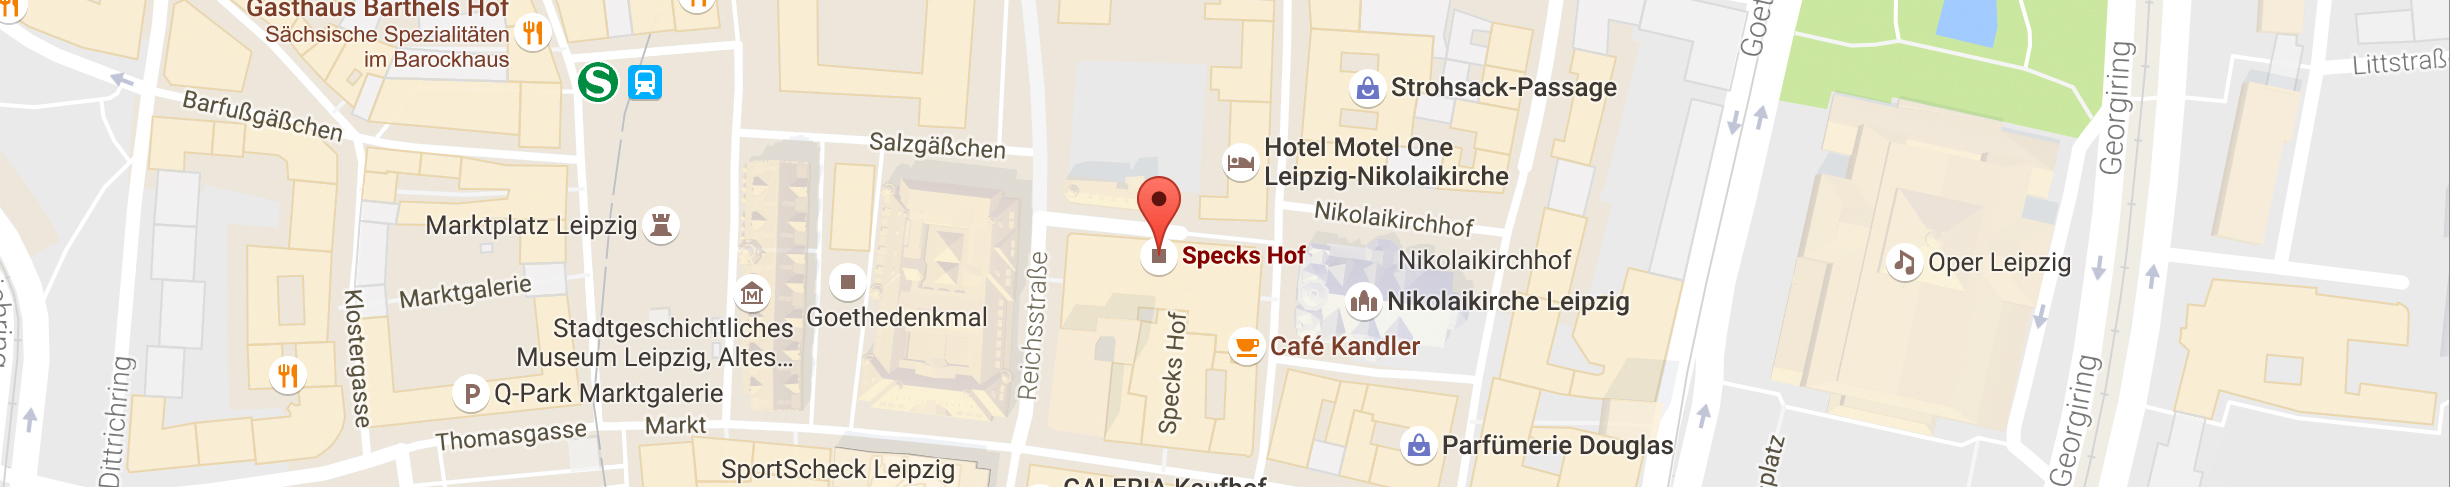
\includegraphics[width=\linewidth]{img/places/sh_map.jpg}
				\caption{Aufnahmeort Speck's Hof}
				\label{img:sh_map}
			\end{figure}
			
	
		\subsubsection{Kameraeinstellungen}
		\begin{minipage}{0.58\textwidth}
			\begin{tabular}{ll}
				Kamera: &Canon EOS 7D \\
				Objektiv: &Canon EF 10-22mm \\
				& F/3.5-4.5 USM\\		
				Brennweite:& 10mm \\
				Belichtungszeit: & $\frac{1}{2}$s / 1s / 1.3s\\
				Blendenwert: & f/8\\
				Empfindlichkeit & ISO 100 \\
			\end{tabular}\\
		\end{minipage}%
		\begin{minipage}{0.42\textwidth}

		\end{minipage}%
		
	\subsubsection{Vorgehen und Fehleranalyse}
	 Die Aufnahmereihe enstand am 05.11.2016 um 16:58 Uhr. Dabei wurde die Kammera nahe dem Eingang platziert und mit einem vertikalen Winkel von 0$^\circ$ mittig auf den Klangbrunnen ausgerichtet. Es wurden sieben Einzelbilder aufgenommen, welche später, zu einem 180$^\circ$ Panorame zusammengesetzt werden. Jedes der Teilbilder wurde mit einem horizontalen Versatz von 30$^\circ$ aufgenommen, sodass diese später, durch das in Punkt \ref{ch:stitiching} beschriebene Stitching, ohne Fehler zusammengefügt werden können. Aufgrund der zuvor durchgeführten Justage des NPP, sind keine Parallaxverschiebungen aufgetreten.
	
	\section{180$^\circ$ Panorama -- Auerbachskeller}
	\label{sec:auer}
	\subsubsection{Aufnahmeort und -idee}
	Einer der Weltweit am bekanntesten Plätze in Leipzig, ist der Auerbachskeller. Er ist die zweitälteste Gaststätte in Leipzig und verdankt seinen Bekanntheitsgrad vorallem Johann Wolfgang von Goethe. Dieser verbrachte hier, während seines Studiums in Leipzig, viele Abende und verewigte ihn schließlich in seinem Werk Faust I in der gleichnamigen Szene \grqq{}Auerbachs Keller in Leipzig\grqq{}. In dieser Szene kommt auch der berühmte Satz \textit{\grqq{}Mein Leipzig lob ich mir! Es ist ein klein Paris und bildet seine Leute.\grqq{}} vor.
	
	\bigskip
	Der Auerbachskeller befindet sich in der Grimmaischen Straße 2–4, direkt unterhalb der Mädlerpassage. Er wird von zwei Statuen eingerahmt, welche 1913 von dem Bildhauer Mathieu Molitor erstellt wurden. Sie zeigen zum Einem Faust zusammen mit Mephisto und zum Anderen drei verzauberte Studenten. Diese befinden sich im Vordergrund und bilden zusammen mit der historischen Passage im Hintergrund ein optimales Motiv für ein 180$^\circ$ Panorama.
	
	\begin{figure}[H]
		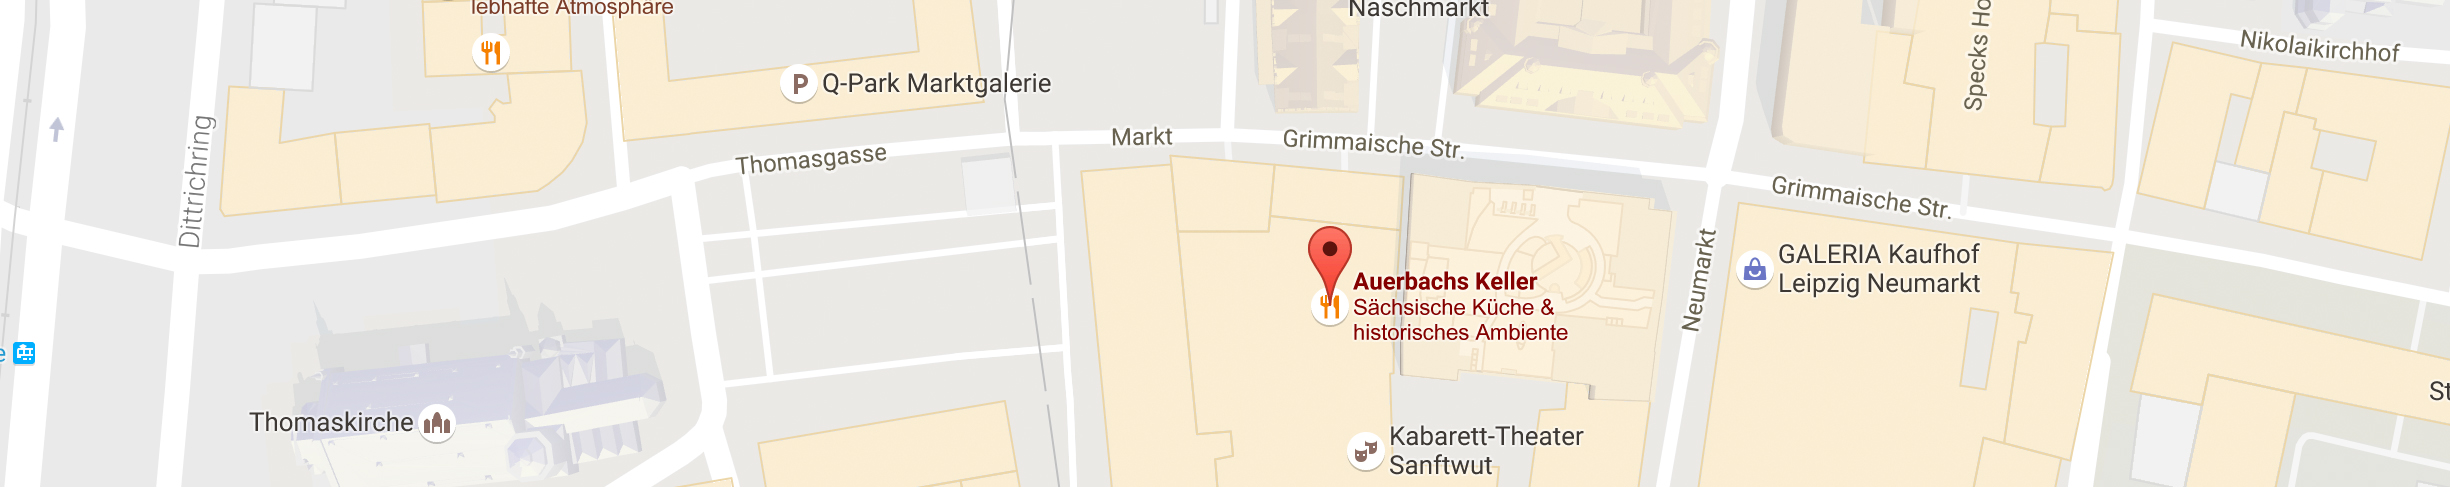
\includegraphics[width=\linewidth]{img/places/ak_map.jpg}
		\caption{Aufnahmeort Auerbachskeller}
		\label{img:ak_map}
	\end{figure}

	\subsubsection{Kameraeinstellungen}
	\begin{minipage}{0.58\textwidth}
		\begin{tabular}{ll}
			Kamera: &Canon EOS 7D \\
			Objektiv: &Canon EF 10-22mm \\
			& F/3.5-4.5 USM\\		
			Brennweite:& 10mm \\
			Belichtungszeit: & 1s / 1.3s / 1.6s / 2s\\
			Blendenwert: & f/8\\
			Empfindlichkeit & ISO 100 \\
		\end{tabular}\\
	\end{minipage}%
	\begin{minipage}{0.42\textwidth}
		\begin{figure}[H]
			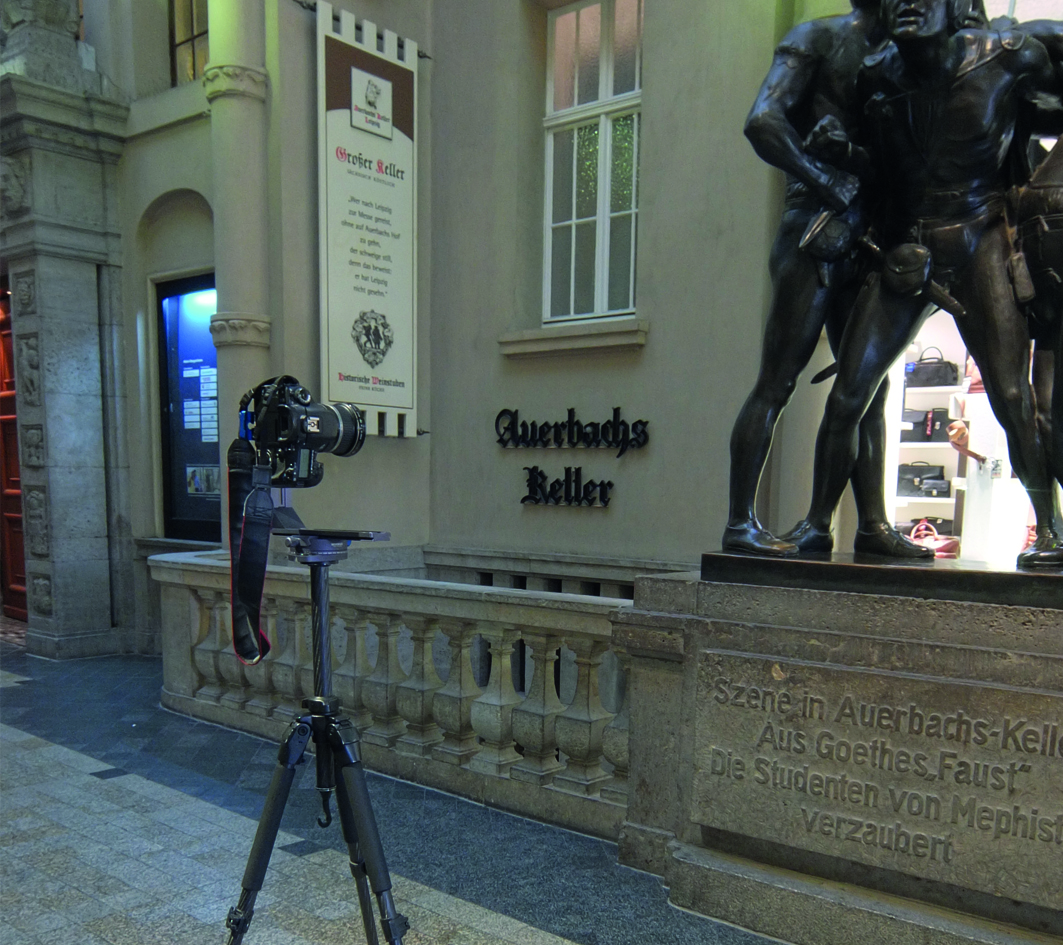
\includegraphics[width=\linewidth]{img/places/ak.jpg}
			\caption{Aufnahmesituation Auerbachskeller}
			\label{img:ak}
		\end{figure}
	\end{minipage}%
	

	
	\subsubsection{Vorgehen und Fehleranalyse}
	Für die Aufnahme der Einzelbilder wurde genauso vorgegangen, wie es bereits unter Punkt \ref{sec:specks} beschrieben. Die Kamera wurde mit einem vertikalen Winkel von 0$^\circ$ mittig zwischen den beiden Statuen positioniert. Diese befinden sich am rechten und linken Rand des 180$^\circ$ Panoramas. Durch einen horizontalen Versatz von 30$^\circ$ entstanden sieben Teilbilder, welche am 05.11.2016 um 17:07 Uhr aufgenommen wurden. 

	\section{180$^\circ$ Nachtpanorama -- Richard Wagner Platz}
	\label{sec:wagner}
	\subsubsection{Aufnahmeort und -idee}
	Der Richard-Wagner Platz befindet sich am nordwestlichen Zugang zur Leipziger Innenstadt. Historisch befand sich an dieser Stelle das Ranstädter Tor, eines der vier Stadttore Leipzigs. Namensgeber war der Komponist Richard Wagner, dessen Geburtshaus sich in unmittelbare Nähe befand.
	
	\bigskip
	Der Platz wird eingerahmt von dem Geschäftshaus \grqq{}Großer Blumenberg\grqq{}, den Höfen am Brühl, dem Goerdlerring und der Evangelisch Reformierte Kirche zu Leipzig. Besonders die Fassade der ehemaligen \grqq{}Blechbüchse\grqq{} ist sehr markant und bildet zusammen mit den vier Springbrunnen, welche sich direkt auf dem Platz befinden einen modernen Gegensatz zur restlichen Altstadt Leipzigs.
	
	\bigskip
	Zahlreiche Geschäfte, Bars und Restaurants sind am Abend beleuchtet und tauchen den Platz in ein angenehmes Licht, mit einer ruhigen  Atmosphäre. Sodass dieser für das 180$^\circ$ Nachtpanorama gewählt wurde.
	
	\begin{figure}[H]
		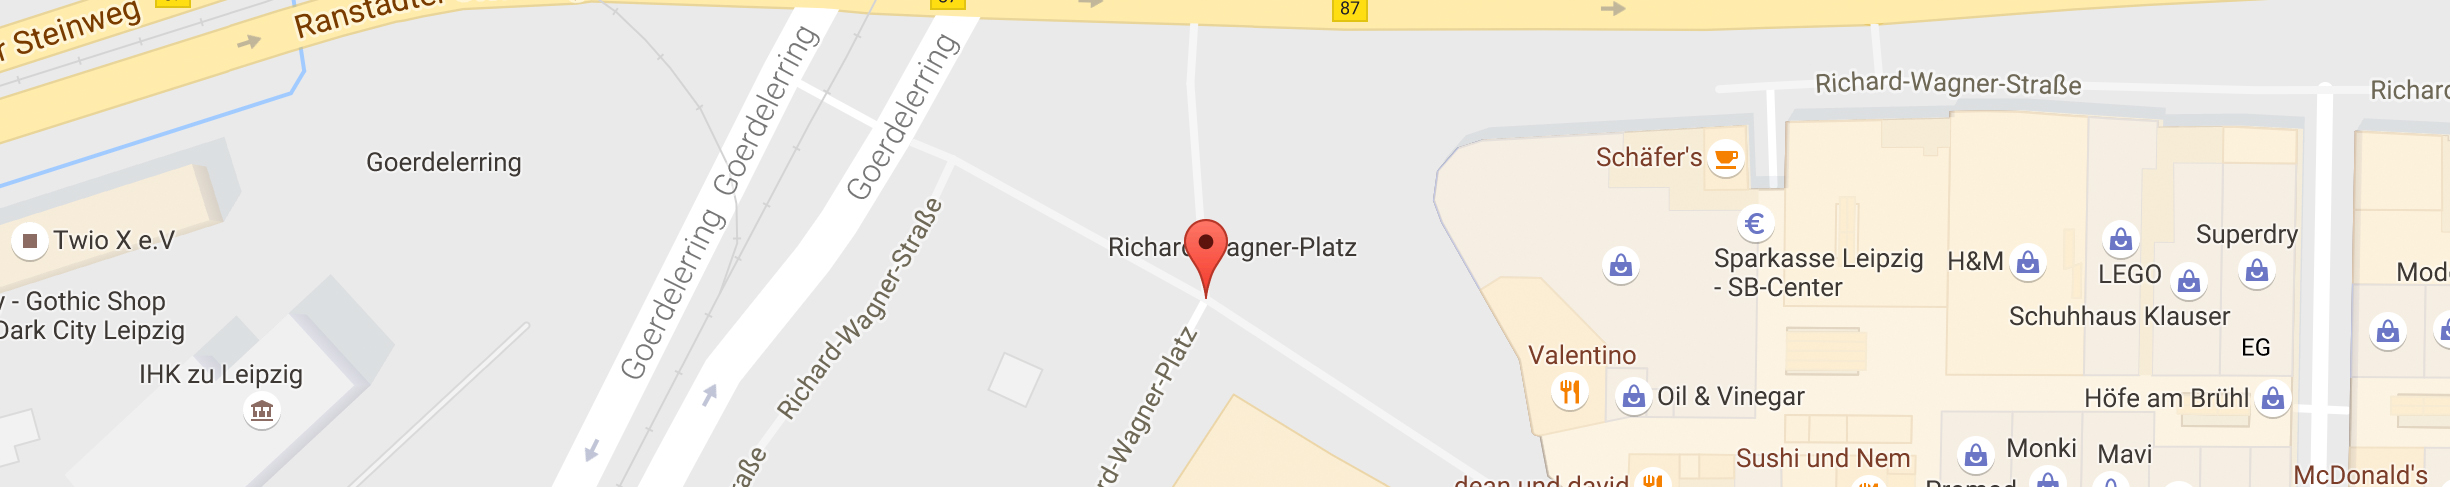
\includegraphics[width=\linewidth]{img/places/rw_map.jpg}
		\caption{Aufnahmeort Richard-Wagner-Platz}
		\label{img:rw_map}
	\end{figure}
	
	\subsubsection{Kameraeinstellungen}
	\begin{minipage}{0.58\textwidth}
	\begin{tabular}{ll}
		Kamera: &Canon EOS 7D \\
		Objektiv: &Canon EF 10-22mm \\
		& F/3.5-4.5 USM\\		
		Brennweite:& 11mm \\
		Belichtungszeit: & 5s / 6s / 8s\\
		Blendenwert: & f/8\\
		Empfindlichkeit & ISO 100 \\
	\end{tabular}\\
	\end{minipage}%
	\begin{minipage}{0.42\textwidth}

	\end{minipage}%
	

			
	\subsubsection{Vorgehen und Fehleranalyse}
	Die vier Teilaufnahmen entstanden am 02.11.2016 um 18:26 Uhr. Zu dieser Zeit war es bereits so dunkel, dass eine entsprechende lange Belichtungszeit von fünf bis acht Sekunden notwendig war. Aufgrund dessen musste darauf geachtet werden, dass sich keine Fahrräder beziehungsweise Autos während der Belichtung durch das Bild bewegen, da deren Licht ansonsten zu dem sogenannten \grqq{}Lightstream-Effekt\grqq{} führen(siehe Abbildung \ref{img:ls}). Die lange Belichtungszeit führt dazu, das sich bewegende Objekt, wie Personen, verschwinden und auf den Einzelbildern kaum vorhanden sind. Starre Elemente hingegen, wie beispielsweise der Springbrunnen im Vorder- und die Gebäude im Hintergrund sind klar erkennbar. 
	
		\begin{figure}[H]
			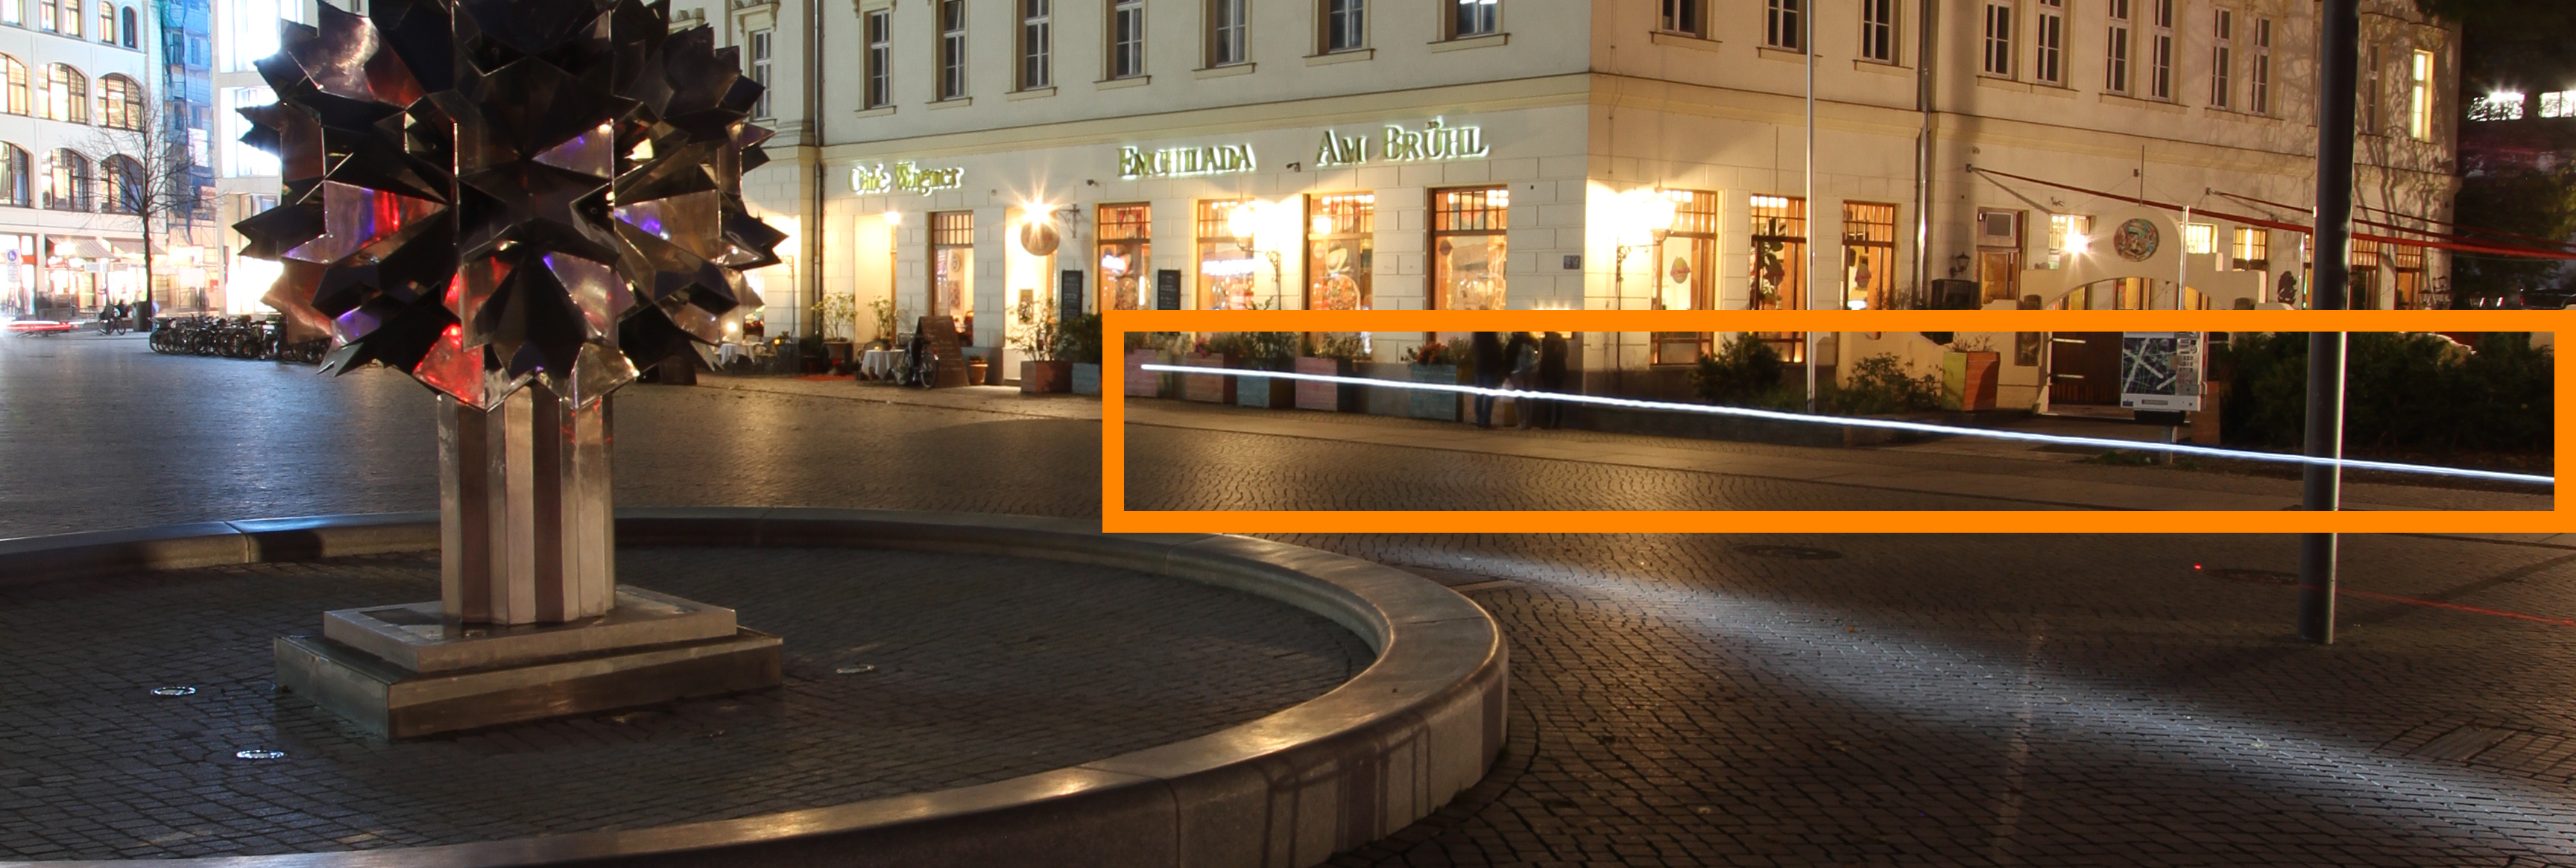
\includegraphics[width=\linewidth]{img/lighstream.jpg}
			\caption{Lightstream Effekt bei langen Belichtungszeiten}
			\label{img:ls}
		\end{figure}
	
	\bigskip
	Die Kamera wurde mit einem vertikalen Winkel von 0$^\circ$  mittig auf dem Platz aufgestellt und in Richtung der Höfe am Brühl ausgerichtet. Die Einzelbilder wurden mit einem Versatz von 45$^\circ$ aufgenommen. Durch die zuvor vorgenommene Justage des NPP treten keine Parallax-Effekte auf. 
	
	\section{360$^\circ$ Panorama -- Augustusplatz}
	\label{sec:augustus}
	\subsubsection{Aufnahmeort und -idee}
	Am östlichen Teil des Leipziger Innenstadtrings befindet sich der Augustusplatz, welcher mit repräsentativen und kulturellen Bauwerken umgeben ist. Die beiden bekanntesten sind das Gewandhaus und die Leipziger Oper, welche sich frontal gegenüberstehen. Unmittelbar vor dem Gewandhaus steht der Mendebrunnen, welcher um 1880 entstand und als letztes historisches Bauwerk dieses Platzes, sowohl Angriffe des zweiten Weltkrieges, als auch Baumaßnahmen der DDR-Zeit überstand. 
	
	\bigskip
	Daneben finden sich unter anderen das City Hochhaus, das neue Augusteum und Paulinum der Universität Leipzig, das Krochhochhaus und die alte Handelspost. Diese prägen das Stadtbild Leipzigs und sorgen dafür, dass der Augustusplatz ideal für ein 360$^\circ$ Panorama geeignet ist.
			\begin{figure}[H]
				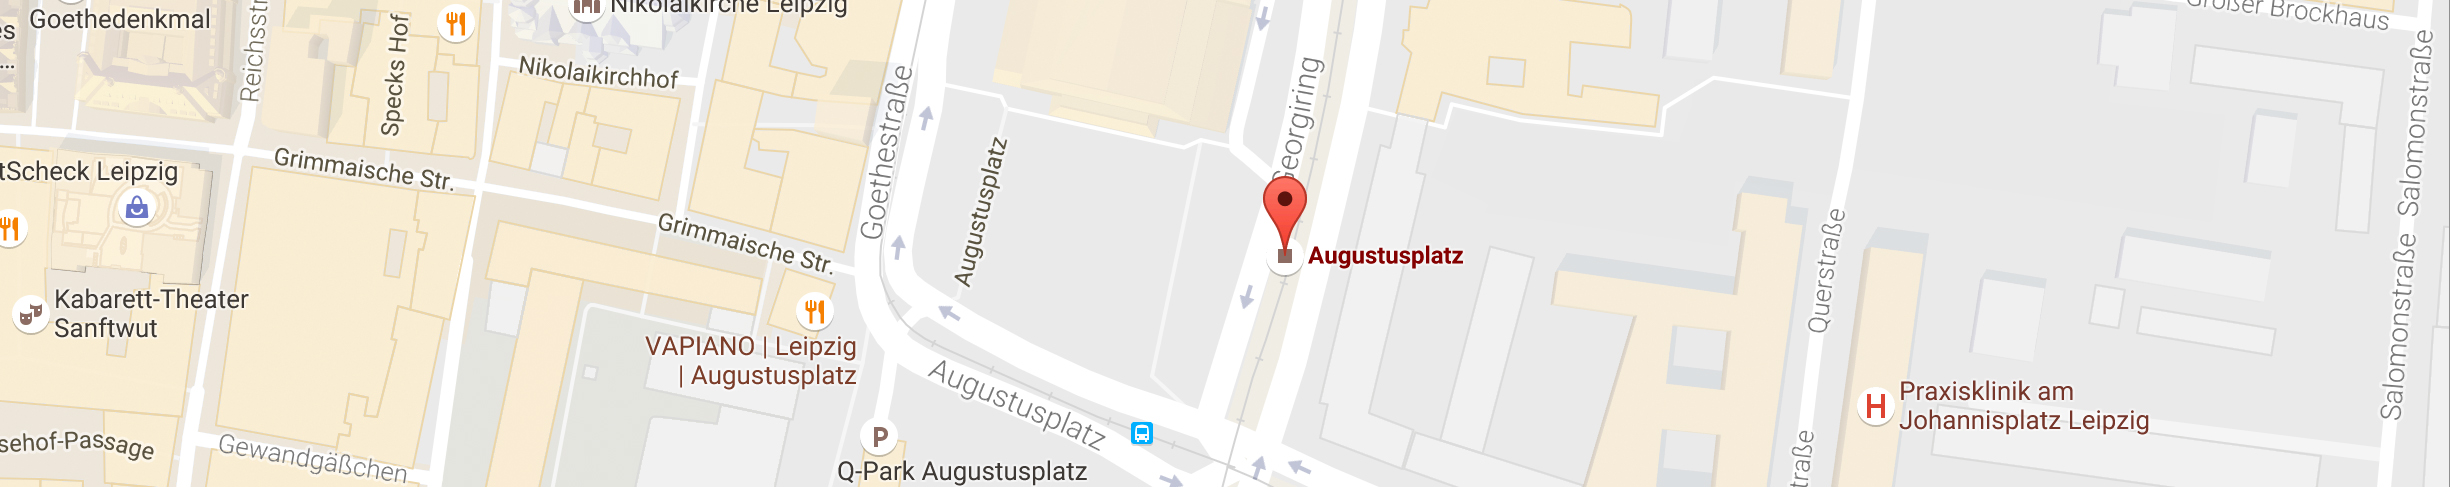
\includegraphics[width=\linewidth]{img/places/ap_map.jpg}
				\caption{Aufnahmeort Augustusplatz}
				\label{img:ak_map}
			\end{figure}
	
		\subsubsection{Kameraeinstellungen}
		\begin{minipage}{0.58\textwidth}
			\begin{tabular}{ll}
				Kamera: &Canon EOS 7D \\
				Objektiv: &Canon EF 10-22mm \\
				& F/3.5-4.5 USM\\		
				Brennweite:& 10mm \\
				Belichtungszeit: &$\frac{1}{40}$s /$\frac{1}{60}$s / $\frac{1}{80}$s / $\frac{1}{100}$s \\
				 &$\frac{1}{125}$s / $\frac{1}{160}$s / $\frac{1}{200}$s \\
				 &$\frac{1}{250}$s / $\frac{1}{400}$s \\
				Blendenwert: & f/8\\
				Empfindlichkeit & ISO 100 \\
			\end{tabular}\\
		\end{minipage}%
		\begin{minipage}{0.42\textwidth}
			\begin{figure}[H]
				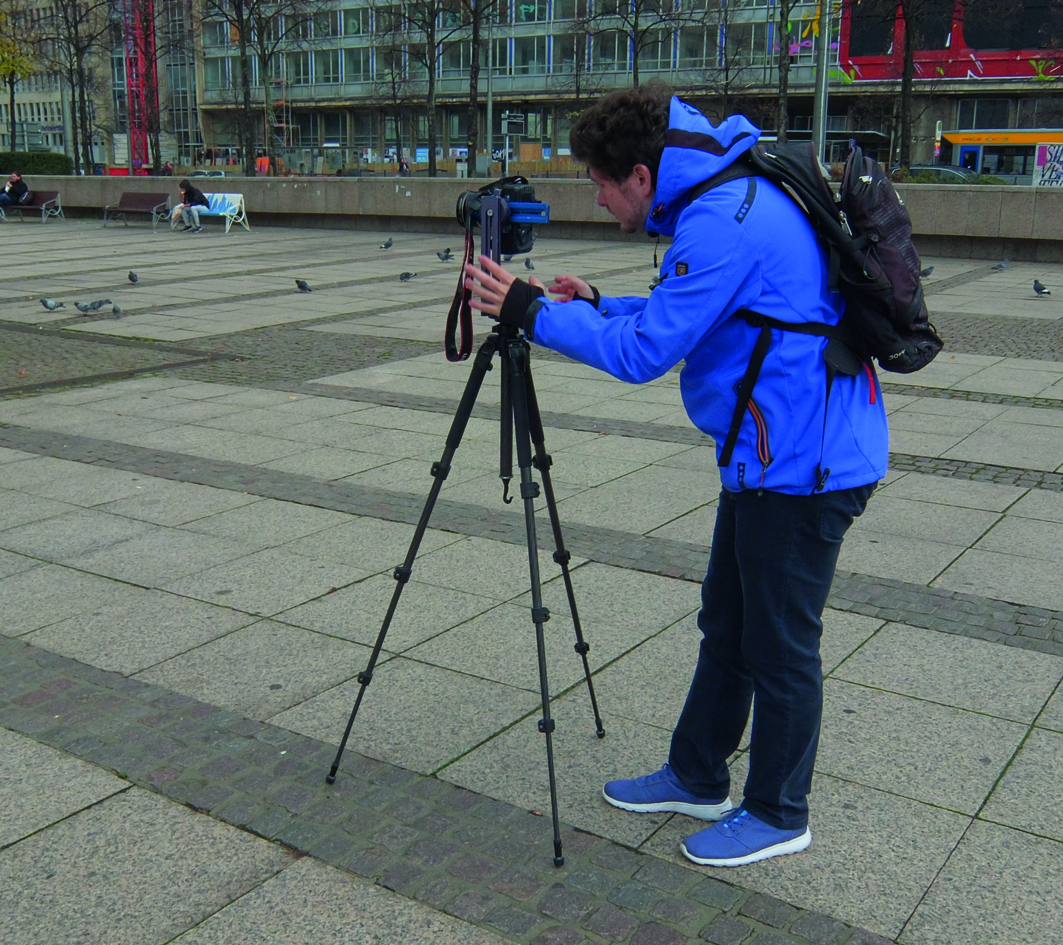
\includegraphics[width=\linewidth]{img/places/ap.jpg}
				\caption{Aufnahmesituation Augustusplatz}
				\label{img:ak}
			\end{figure}
		\end{minipage}%
		
	\subsubsection{Vorgehen und Fehleranalyse}
	Um dieses 360$^\circ$ Panorama zu erstellen, wurden am 02.11.2016 um 14:53 Uhr, 13 Einzelaufnahmen angefertigt, welche einen horizontalen Versatz von jeweils 30$^\circ$ haben. Zuvor wurde die Kamera nicht mittig auf dem Platz, sondern nahe dem Mendebrunnen aufgestellt und mittig zum neuen Paulinum ausgerichtet. Beim späteren stitchen wurden die Anordnung der Bilder allerdings so verändert, dass die Oper als zentrales Objekt innerhalb des Panoramas platziert ist. 
	
	\bigskip
		Aufgrund des sehr wechselhaften Wetters mussten die 13 Teilbilder zügig hintereinander aufgenommen werden. Wobei aufgrund des Wechsels von Sonne und Wolken immer wieder die Belichtungszeit angepasst werden musste. Durch die genaue Justage des No Parallax Point, treten im späteren 360$^\circ$ Panorama keine Parallax-Effekte auf. Das Stitching konnte problemlos durchgeführt werden, ohne dass falsche Überlappungen oder Verschiebungen auftreten, was besonders gut an dem kleinteiligen Boden erkennbar ist.

	
	\section{360$^\circ$ Nachtpanorama -- Marktplatz}
	\label{sec:markt}
		\subsubsection{Aufnahmeort und -idee}
		Leipzigs Marktplatz bildet das Zentrum der Leipziger Innenstadt. Er ist ringsum, sowohl mit historischen, als auch modernen Gebäuden bebaut und bietet somit einen architektonischen Mix aus Alt und Neu. So finden sich an diesem Platz beispielsweise die Alte Waage, das Königshaus und Barthels Hof. Das älteste Bauwerk ist das Alt Rathaus, welches 1556 errichtet wurde. Eine Besonderheit bildet der Rathausturm, welcher dieses asymmetrisch, im Goldenen Schnitt unterteilt. 
		
		\bigskip
		Auf dem Marktplatz herrscht immer reges Treiben, aber in den Abendstunden kommt er zur Ruhe. Durch zahlreichen Geschäfte und Restaurants, die sich um den Platz verteilen wird er in ein warmes, indirektes Licht getaucht, sodass eine ruhige und angenehme Atmosphäre entsteht. Aufgrund dessen und der architektonischen Abwechslung eignet sich der Marktplatz besonders für ein 360$^\circ$ Nachtpanorama.
		\begin{figure}[H]
			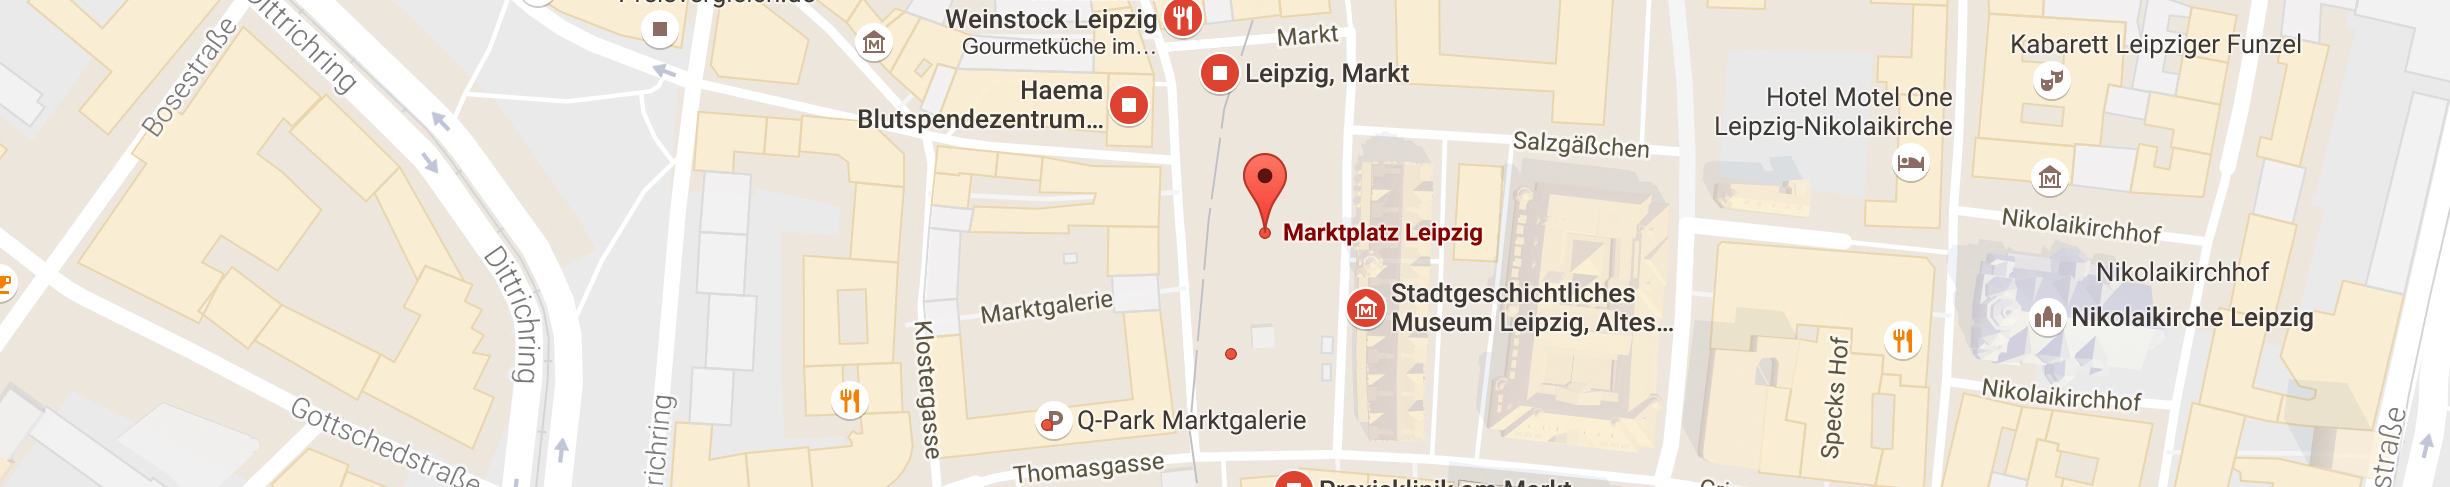
\includegraphics[width=\linewidth]{img/places/mp_map.jpg}
			\caption{Aufnahmeort Marktplatz}
			\label{img:mp_map}
		\end{figure}
		
		\subsubsection{Kameraeinstellungen}
		\begin{minipage}{0.58\textwidth}
			\begin{tabular}{ll}
				Kamera: &Canon EOS 7D \\
				Objektiv: &Canon EF 10-22mm \\
				& F/3.5-4.5 USM\\		
				Brennweite:& 10mm \\
				Belichtungszeit: &1.6s / 2s / 2.5s \\
					& 3.2s / 4s / 5s / 6s \\
					& 8s \\
				Blendenwert: & f/8\\
				Empfindlichkeit & ISO 100 \\
			\end{tabular}\\
		\end{minipage}%
		\begin{minipage}{0.42\textwidth}
			\begin{figure}[H]
				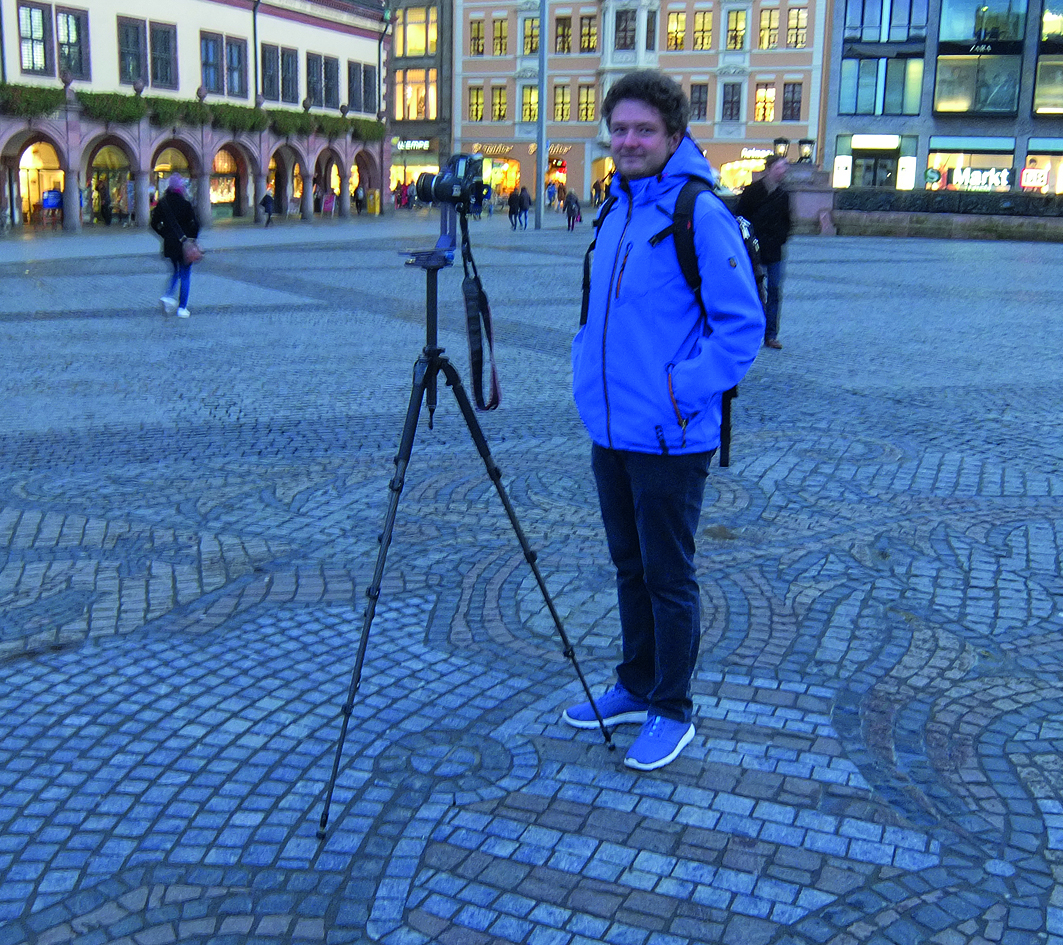
\includegraphics[width=\linewidth]{img/places/mp.jpg}
				\caption{Aufnahmesituation Marktplatz}
				\label{img:mp}
			\end{figure}
		\end{minipage}%
		
		\subsubsection{Vorgehen und Fehleranalyse}
		Am 02.11.2016 um 18:14 Uhr dreizehn Einzelaufnahmen um dieses 360$^\circ$ Nachtpanorama zu realisieren. Dabei wurde auf den richtigen Zeitpunkt gewartet um die Bilder während der Blauen Stunde aufzunehmen. Die Blaue Stunde bezeichnet dabei die Zeit während des Sonnenuntergangs und der Dunkelheit, in welcher der Himmel in ein tiefes Blau gefärbt ist und in etwa die gleiche Helligkeit besitzt wie das  künstliches Licht der umgebenen Gebäude. Es wurden mehrere Testaufnahmen gemacht um den perfekten Zeitpunkt zu erwischen(siehe Abbildung \ref{img:bs}).
		
		\begin{figure}[H]
			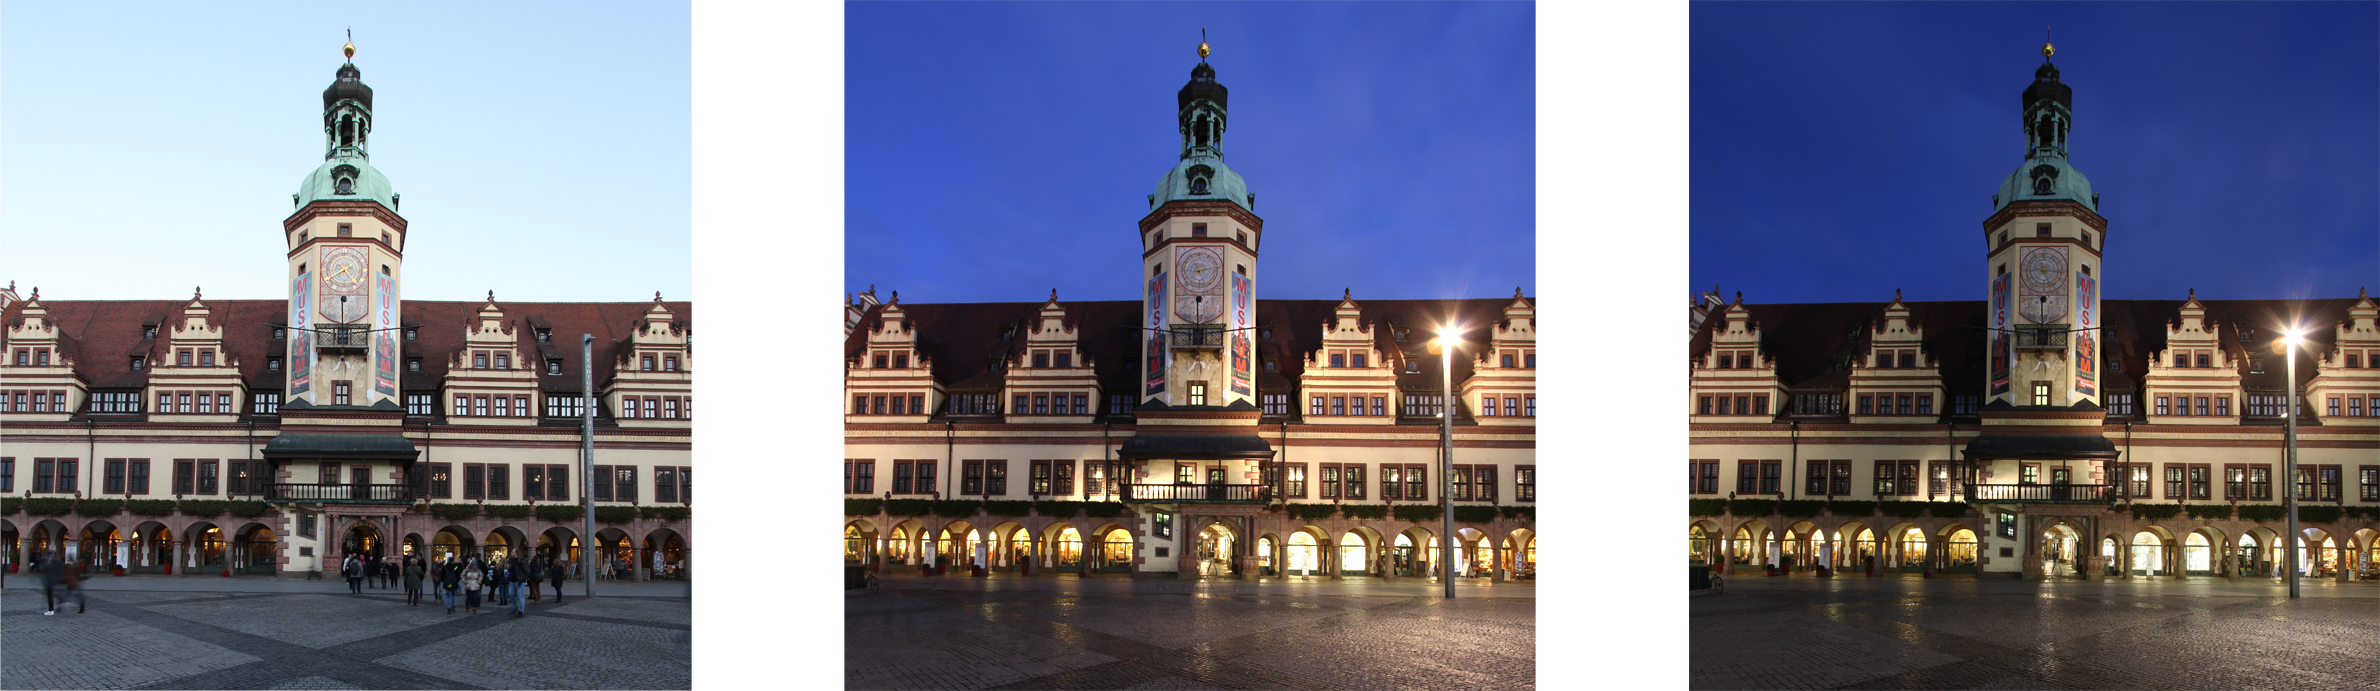
\includegraphics[width=\linewidth]{img/bs.jpg}
			\caption{Blaue Stunde - Testaufnahmen}
			\label{img:bs}
		\end{figure}
		
		Die Kamera wurde mittig zum Rathausturm aufgestellt und auf diesen mit einem vertikalen Winkel von 0$^\circ$ zentral ausgerichtet. Alle weiteren Bilder wurden mit einem horizontalen Versatz von 30$^\circ$ aufgenommen. Durch die zuvor durchgeführte Justage des NPP tritt beim späteren Stitching kein Parallax-Fehler auf. 
		
		\bigskip
		Ähnlich wie im Punkt \ref{sec:wagner} bereits beschrieben besteht durch die lange Belichtungszeit die Gefahr eines Lightstream-Effektes, wie in Abbildung \ref{img:ls-m}. Also musste darauf geachtet werden, dass sich während der Aufnahme kein Fahrrad beziehungsweise Auto durch das Bild bewegt und unter Umständen Aufnahmen wiederholt werden. 

		\begin{figure}[H]
			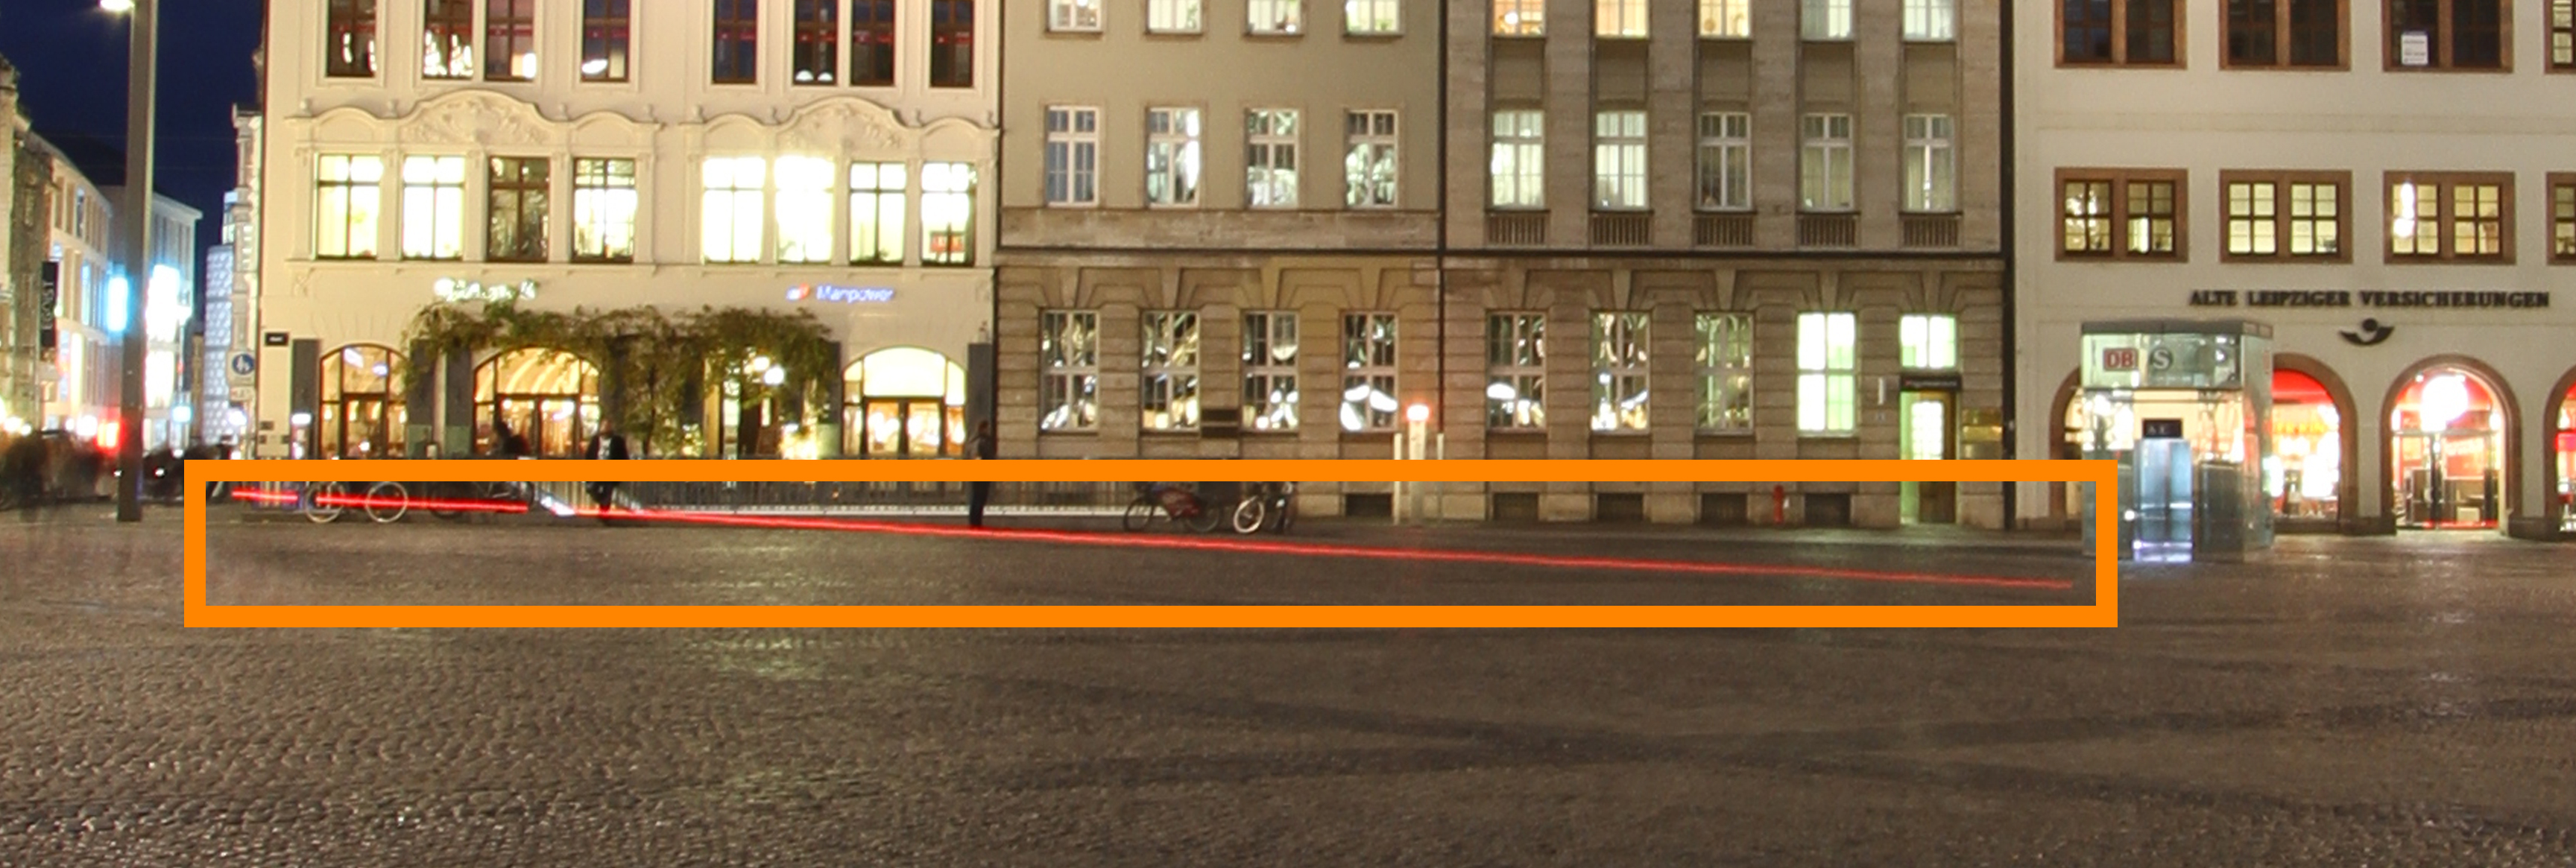
\includegraphics[width=\linewidth]{img/ls-m.jpg}
			\caption{Lightstream Effekt Marktplatz}
			\label{img:ls-m}
		\end{figure}

	\section{Kugelpanorama --  Mädler-Passage}
	\label{sec:kugel}
			\subsubsection{Aufnahmeort und -idee}
			
			\begin{figure}[H]
				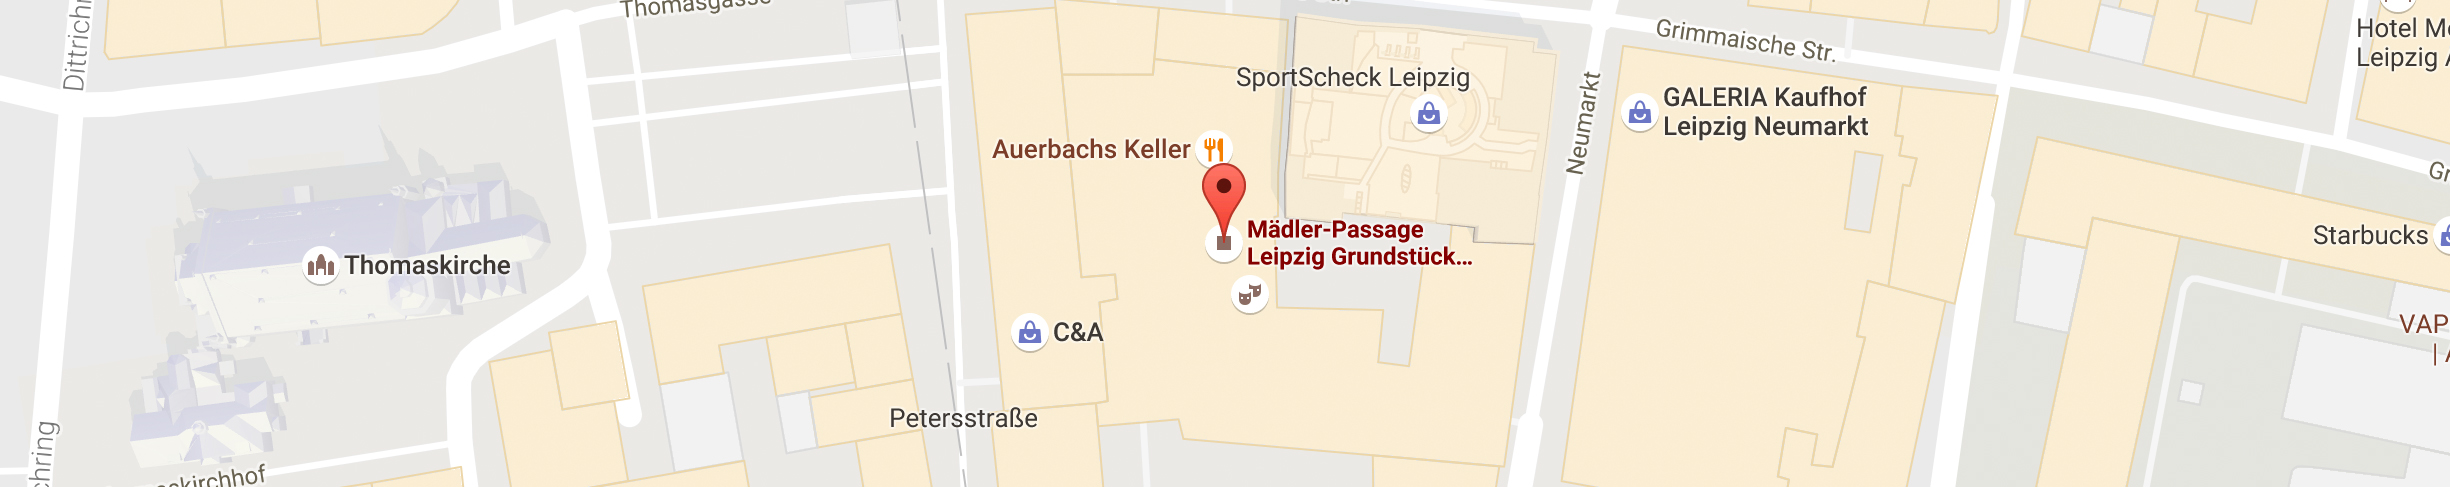
\includegraphics[width=\linewidth]{img/places/mae_map.jpg}
				\caption{Aufnahmeort Mädler-Passage}
				\label{img:mae_map}
			\end{figure}
			
			\subsubsection{Kameraeinstellungen}
			\begin{minipage}{0.58\textwidth}
				\begin{tabular}{ll}
					Kamera: &Canon EOS 7D \\
					Objektiv: &Canon EF 10-22mm \\
					& F/3.5-4.5 USM\\		
					Brennweite:& 10mm \\
					Belichtungszeit: &$\frac{1}{40}$s /$\frac{1}{60}$s / $\frac{1}{80}$s / $\frac{1}{100}$s \\
					&$\frac{1}{125}$s / $\frac{1}{160}$s / $\frac{1}{200}$s \\
					&$\frac{1}{250}$s / $\frac{1}{400}$s \\
					Blendenwert: & f/8\\
					Empfindlichkeit & ISO 100 \\
				\end{tabular}\\
			\end{minipage}%
			\begin{minipage}{0.42\textwidth}
				\begin{figure}[H]
					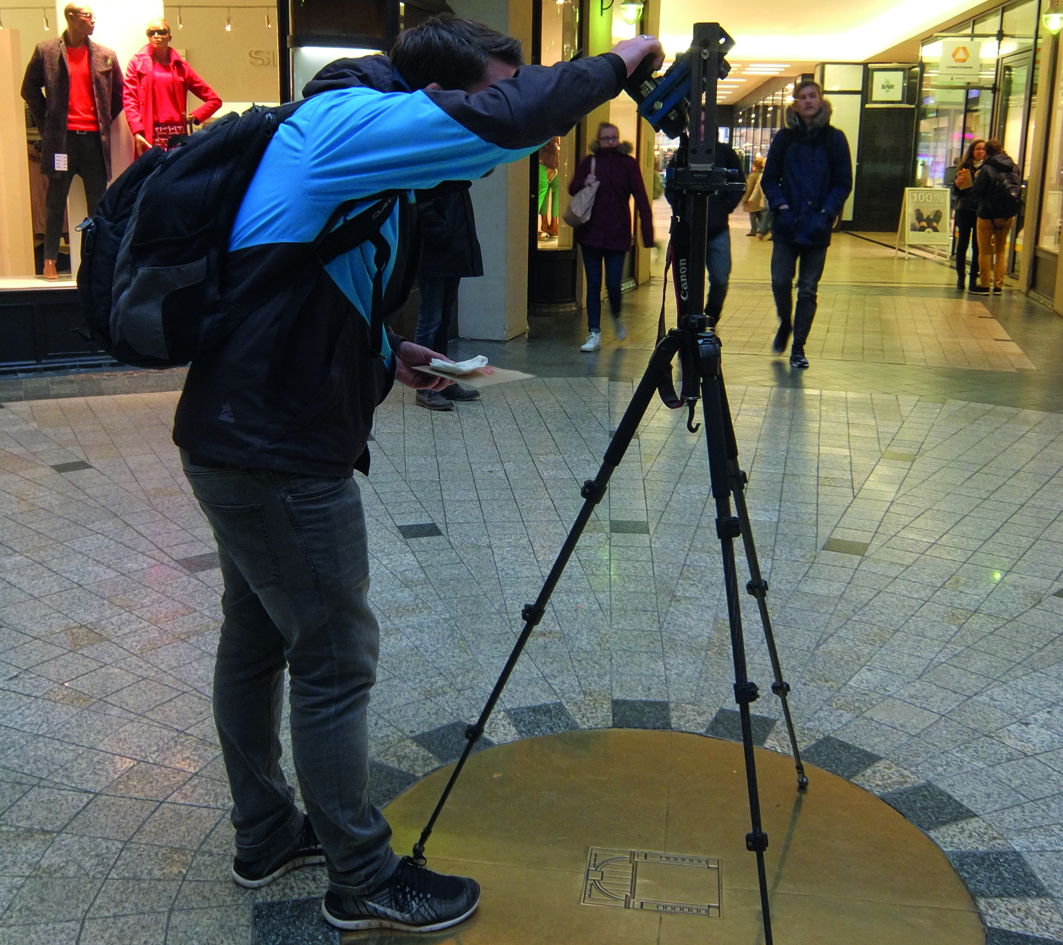
\includegraphics[width=\linewidth]{img/places/mae.jpg}
					\caption{Aufnahmesituation  Mädler-Passage}
					\label{img:ak}
				\end{figure}
			\end{minipage}%
			
			\subsubsection{Vorgehen und Fehleranalyse}
			
			
	\chapter{Stitching}
	\label{ch:stitiching}
	Für ein Panorama aufgenommene Einzelbilder werden in der digitalen Fotografie mittels des sogenannten Stitchings zu einem Gesamtbild zusammengesetzt. Um diesen Vorgang weitestgehend zu automatisieren, gibt es verschiedene kostenlose oder auch kostenpflichtige Programme. In dieser Arbeit wird dabei näher auf Photoshop (\ref{sec:photoshop}) und PTGui Pro (\ref{sec:ptgui}) eingegangen, da diese für die Erstellung und Bearbeitung im Vordergrund stehen. Eine freie Softwarealternative für das Stitchen ist Hugin, welches in dieser Arbeit allerdings keine Verwendung findet, da die eben genannten Alternativen bereits alle benötigten Funktionen beherrschen.
	
	\section{PTGUI Pro}
	\label{sec:ptgui}
	
	Beim Start der Anwendung öffnet sich ein simpel gestaltetes Fenster, welches in Abb. \ref{img:ptgui_step_1} zu sehen ist. Die Software ist übersichtlich in Tabs aufgebaut, welche nach dem Laden der Fotos verschiedene Optionen bereitstellen. Mit einem Klick auf \grqq{}Advanced\grqq{} lassen sich diese noch erweitern.
	\begin{figure}[H]
		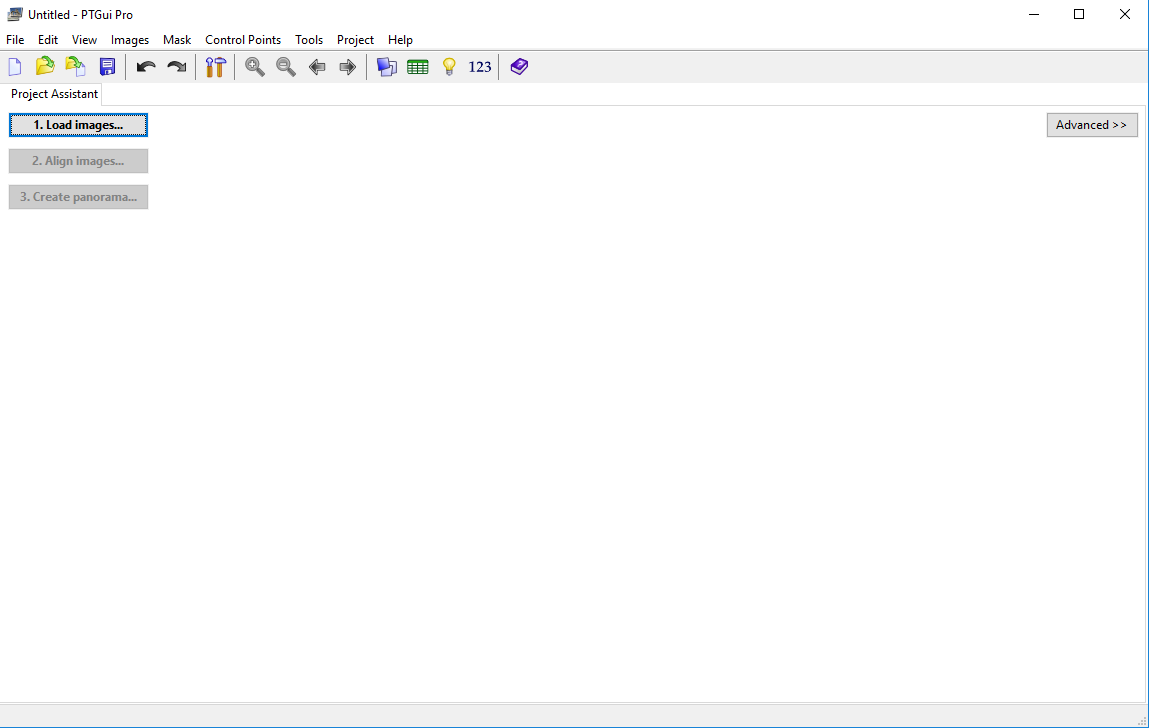
\includegraphics[width=\linewidth]{img/steps/PTGui_Step_1.PNG}
		\caption{PTGui Pro: Startfenster}
		\label{img:ptgui_step_1}
	\end{figure}
	\bigskip
	Über den \grqq{}Load images... -- Button\grqq{} lassen sich die Quellbilder zu einem neuen Projekt hinzufügen. Auch können an dieser Stelle Belichtungsreihen für die HDR--Entwicklung importiert werden. Anschließend werden die geladenen Bilder in dem bereits beschriebenen Startfenster angezeigt und die Einstellungsoptionen werden in Form von Tabs oberhalb angeordnet. Wie aus Abb. \ref{img:ptgui_step_2} weiter hervorgeht, erkennt PTGui automatisch die verwendete Brennweite und den Cropfaktor. Beide Angaben lassen sich zudem manuell einfügen. Unter dem Tab \grqq{}Source Images\grqq{} lässt sich ua. auch die Reihenfolge der Bilder festlegen.
	\begin{figure}[H]
		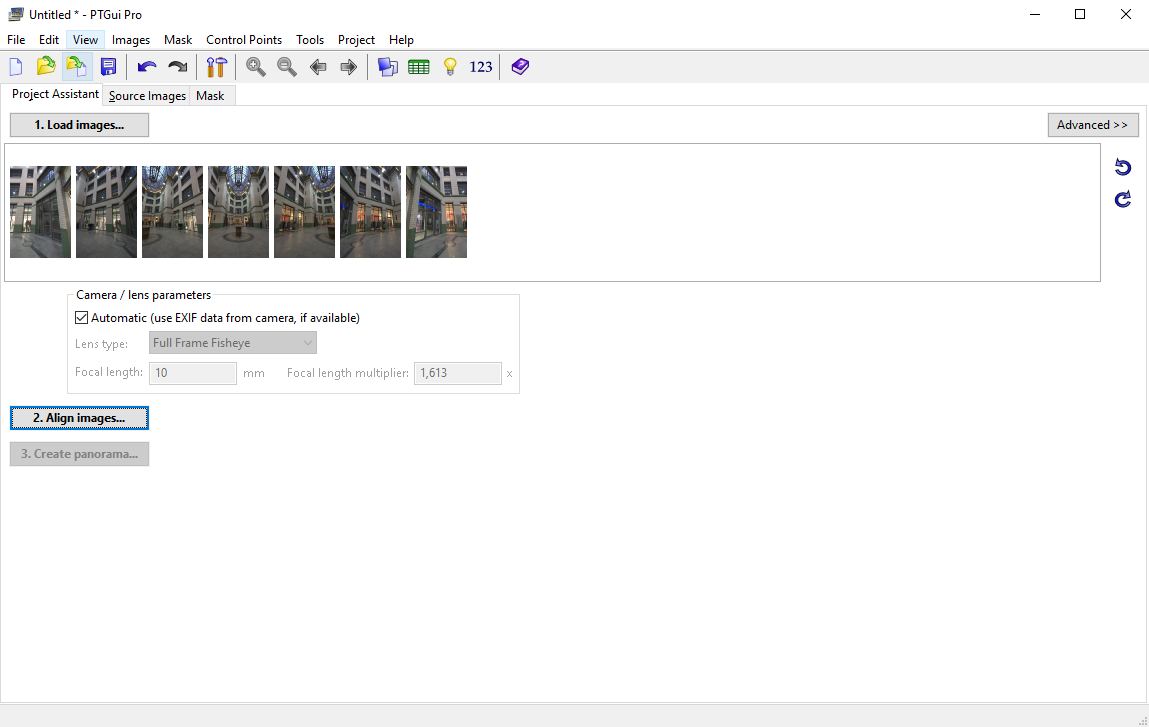
\includegraphics[width=\linewidth]{img/steps/PTGui_Step_2.PNG}
		\caption{PTGui Pro: Laden der Fotos}
		\label{img:ptgui_step_2}
	\end{figure}
	\bigskip
	Sind die erweiterten Einstellungen aktiviert, kann der Benutzer der Software zusätzliche manuelle, kameraspezifische Konfigurationen vornehmen s. Abb. \ref{img:ptgui_step_3}.
	\begin{figure}[H]
		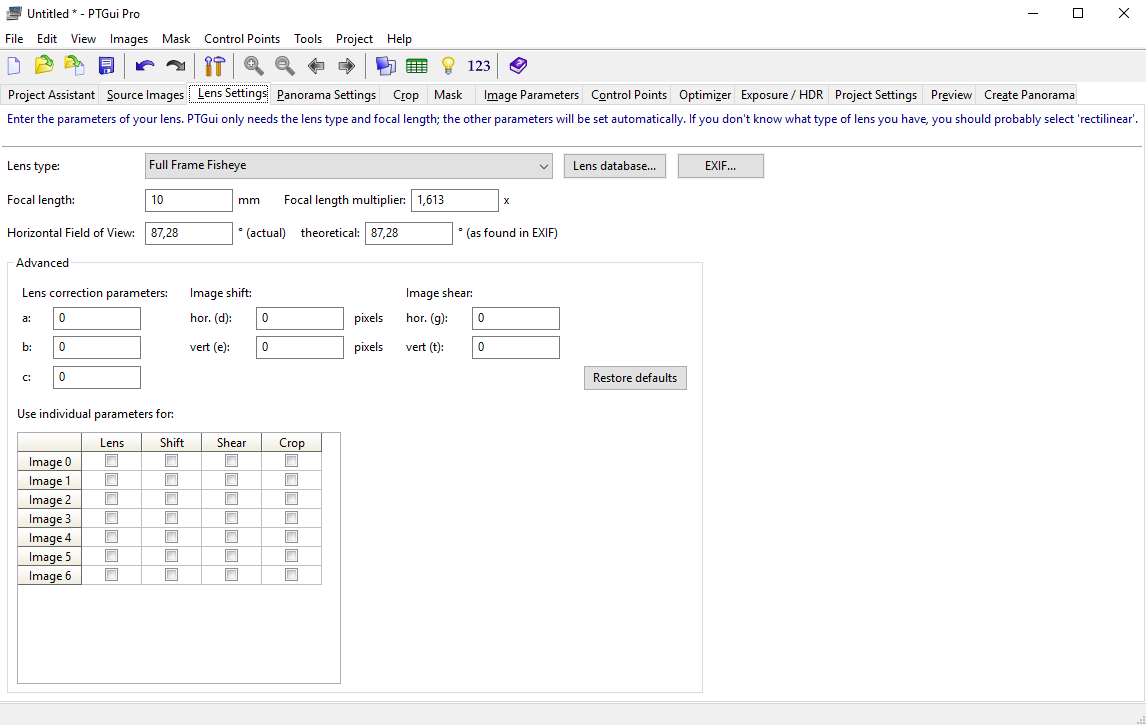
\includegraphics[width=\linewidth]{img/steps/PTGui_Step_3.PNG}
		\caption{PTGui Pro: Objektiveinstellungen}
		\label{img:ptgui_step_3}
	\end{figure}
	\bigskip
	Mit einem Klick auf \grqq{}Align Images\grqq{} beginnt die Software mit dem Stitching der Einzelbilder. Anschließend öffnet sich ein weiteres Fenster, auf welchem das zusammengefügte Panorama betrachten lässt. Zudem werden den bereits bestehenden Tabs weitere angefügt s. Abb. \ref{img:ptgui_step_4}. 
	\begin{figure}[H]
		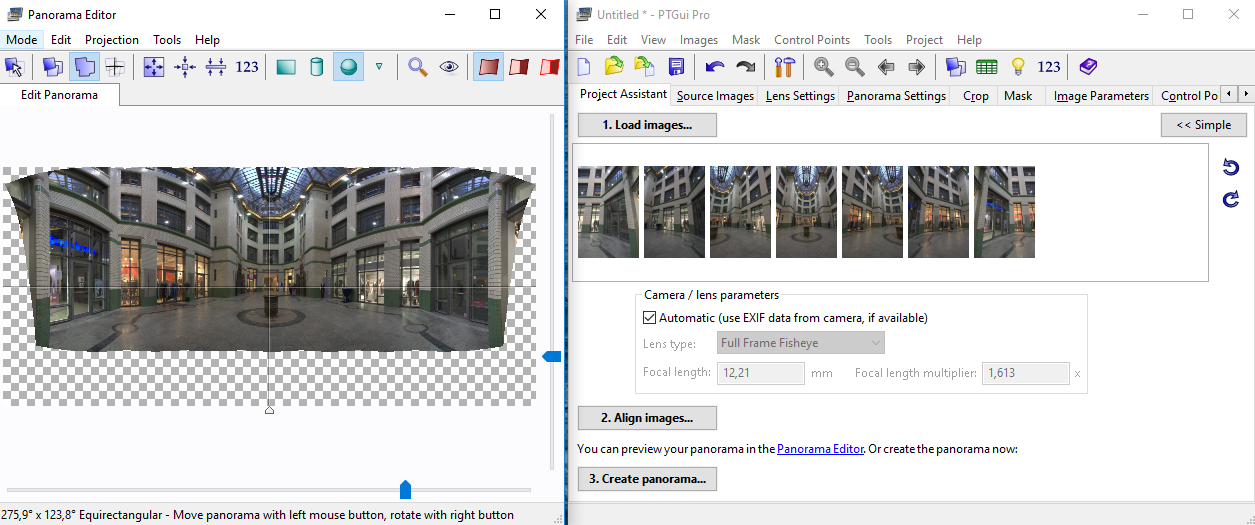
\includegraphics[width=\linewidth]{img/steps/PTGui_Step_4.PNG}
		\caption{PTGui Pro: Panoramaerstellung}
		\label{img:ptgui_step_4}
	\end{figure}
	\bigskip
	Wie in Abb. \ref{img:ptgui_step_4_1} zu sehen ist, kann man mit Hilfe der Maskierung in PTGui Pro, Bereiche kennzeichnen. Diese Markierungen geben an, ob diese Bereiche vom Foto im fertigen Panorama vorhanden (grün) oder nicht  vorhanden (rot) sein sollen. Die Software versucht diesem Wunsch nachzukommen und nimmt für rot markierte Bereiche überlappende Teile aus dem Nachbarbild und fügt diese stattdessen ein.
	\begin{figure}[H]
		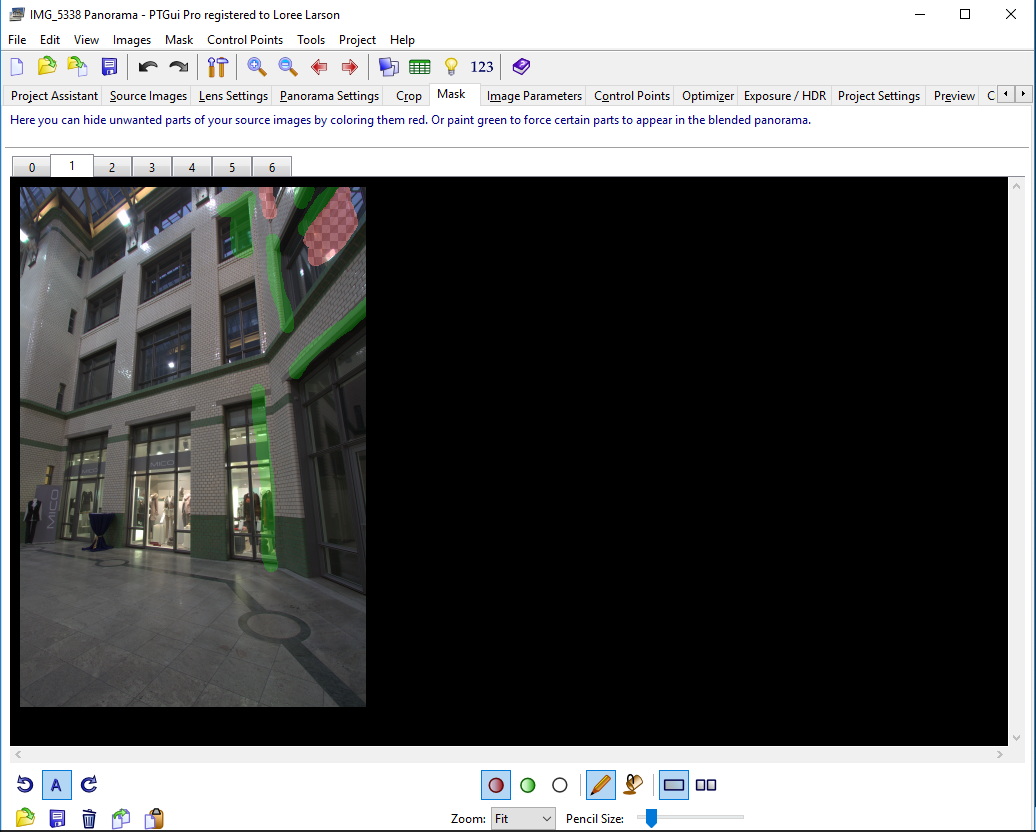
\includegraphics[width=\linewidth]{img/steps/PTGui_Step_4_1.PNG}
		\caption{PTGui Pro: Maskierung}
		\label{img:ptgui_step_4_1}
	\end{figure}
	\bigskip
	Zudem bietet die Software die Möglichkeit für die jeweils zusammengefügten Fotos die sog. Kontrollpunkte zu überprüfen, verändern oder neue zu setzen. Mittels dieser bestimmt die Software, an welchen Stellen die beiden Bilder zusammengefügt werden. Dies ist in Abb. \ref{img:ptgui_step_5} zu sehen. Ein Kontrollpunkt auf dem linken Foto muss dabei einen auf dem rechten Bild entsprechen.
	\begin{figure}[H]
		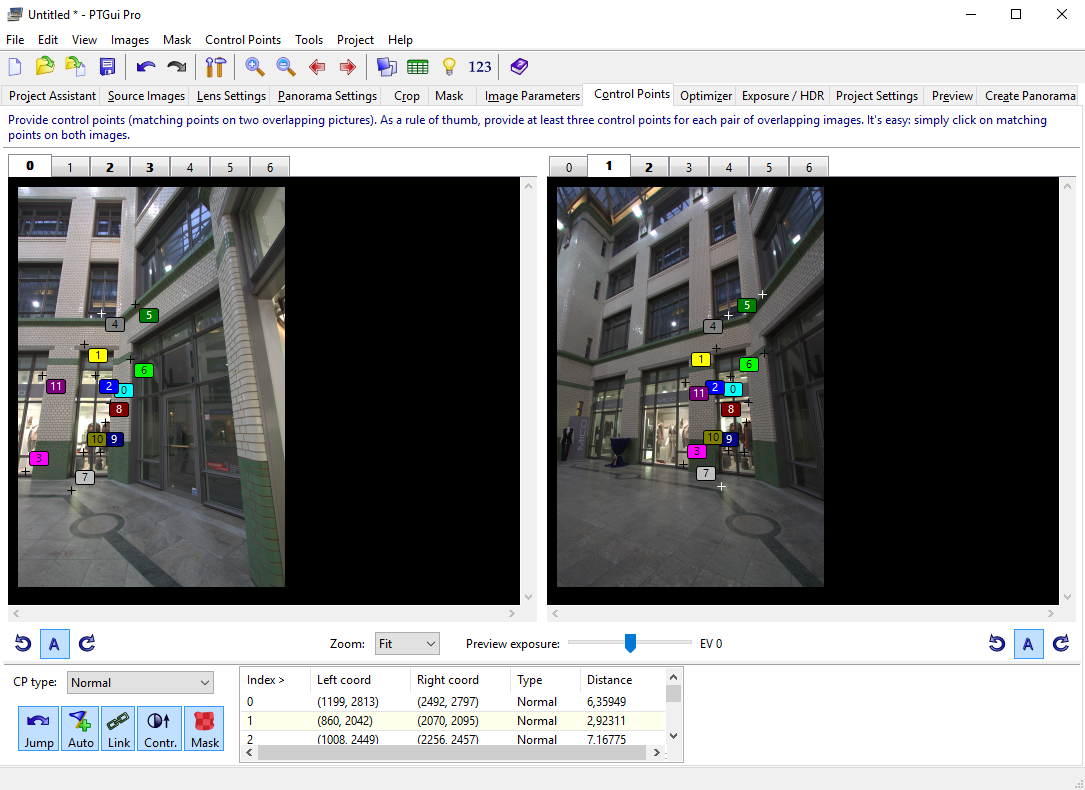
\includegraphics[width=\linewidth]{img/steps/PTGui_Step_5.PNG}
		\caption{PTGui Pro: Kontrollpunkte}
		\label{img:ptgui_step_5}
	\end{figure}
	\bigskip
	Um die Änderung der Ausrichtung vom Bild zu übernehmen, muss der \grqq{}Optimizer\grqq{} im nächsten Tab ausgeführt werden s. Abb. \ref{img:ptgui_step_6}.
	\begin{figure}[H]
		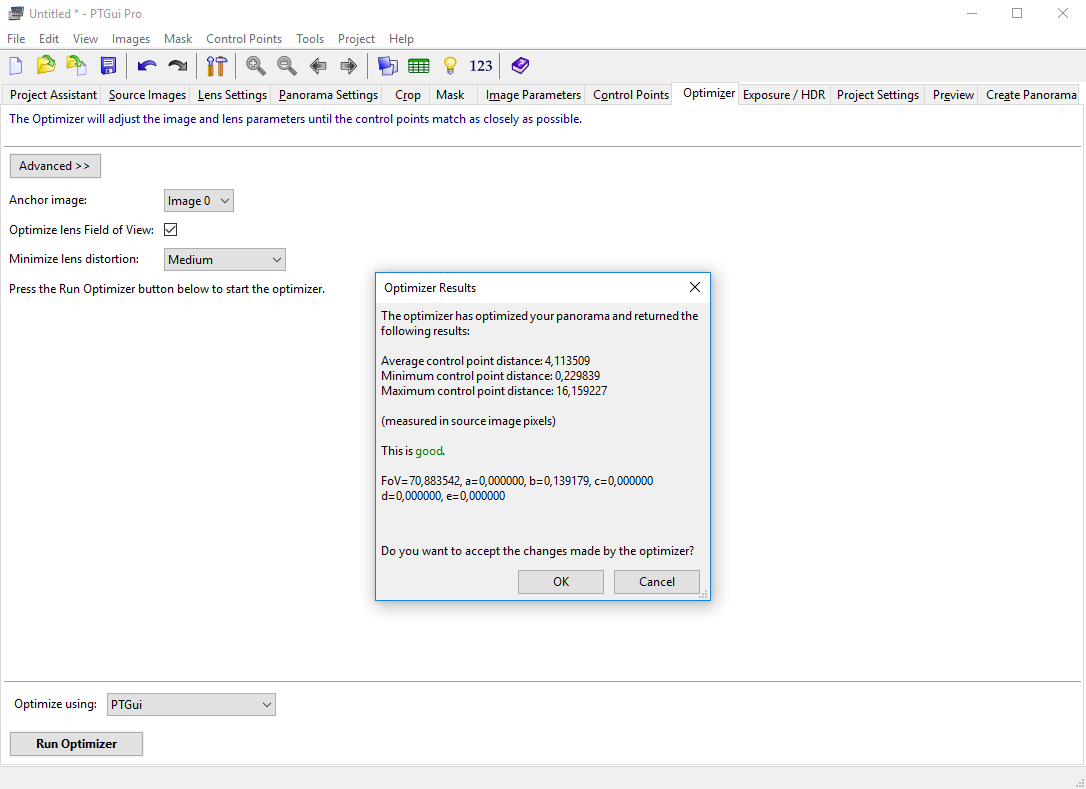
\includegraphics[width=\linewidth]{img/steps/PTGui_Step_6.PNG}
		\caption{PTGui Pro: Optimierung}
		\label{img:ptgui_step_6}
	\end{figure}
	\bigskip
	Nach all diesen Schritten, kann das Panorama exportiert werden s. Abb. \ref{img:ptgui_step_7}. Für dieses Projekt wird das Panorama im TIFF-Format gespeichert, um es in der Nachbearbeitung möglichst verlustfrei korrigieren zu können. Durch einen Klick auf \grqq{}Create Panorama\grqq{} wird der Speichervorgang gestartet. Alternativ ist es auch möglich zusätzlich eine Projektdatei anzulegen, welche für eventuelle, nachträgliche Korrekturen geladen werden kann. 
	\begin{figure}[H]
		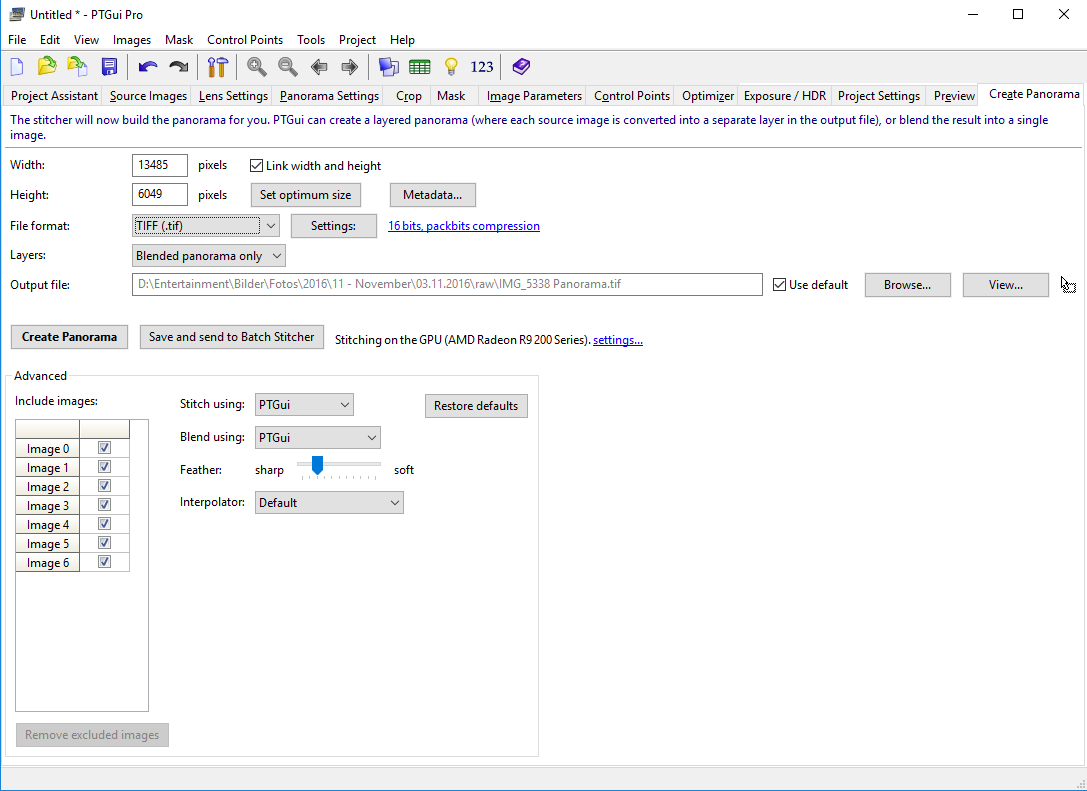
\includegraphics[width=\linewidth]{img/steps/PTGui_Step_7.PNG}
		\caption{PTGui Pro: Export}
		\label{img:ptgui_step_7}
	\end{figure}
	
	\section{Adobe Photoshop}
	\label{sec:photoshop}
	Adobe Photoshop beinhaltet das Tool \grqq{}Photomerge\grqq{}, mit dessen Hilfe Bilderreihen zu Panoramas zusammengefügt werden können. Dieses Kapitel befasst sich deswegen mit dem Stitching mittels Photoshop, wobei zugleich das Programm PTGui Pro (Kap. \ref{sec:ptgui}) als Vergleich herbeigezogen wird.
	\bigskip
	Das Tool Photomerge ist über das Menü unter Datei, Automatisieren zu erreichen. Nach dem Starten öffnet sich ein neues Fenster mit mehreren Einstellungsmöglichkeiten s. Abb. \ref{img:photoshop_step_2}.
	In dieser Ansicht kann auf der linken Seite der gewünschte Panoramatyp mittels einer Checkbox ausgewählt werden. In der Mitte befindet sich der Fotoimport. Es werden alle gängigen Bildformate unterstützt, auch RAW-Dateien. Zusätzliche Korrekturen, wie Vignettierungsentfernung, Verzerrungskorrektur und Auffüllung von Leerbereichen sind auswählbar. Im Gegensatz zu PTGui Pro sind keine weiteren Einstellungsmöglichkeiten vorhanden. Mit der Bestätigung auf \grqq{}OK\grqq{} erstellt Photomerge selbstständig und automatisiert ein Panorama.
	\begin{figure}[H]
		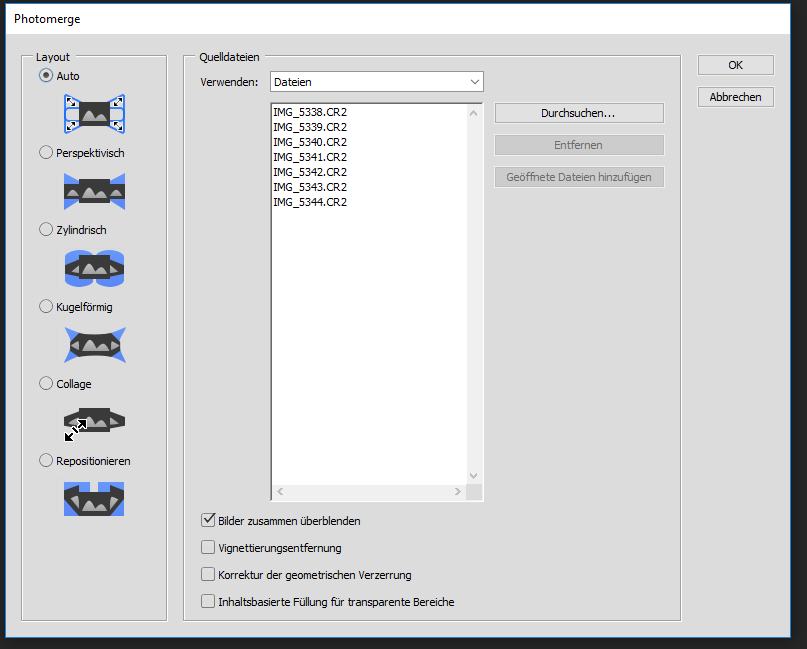
\includegraphics[width=\linewidth]{img/steps/Photoshop_Step_2.png}
		\caption{Photomerge: Startbildschirm}
		\label{img:photoshop_step_2}
	\end{figure}
	\bigskip

	Photomerge lädt die Fotos während des Stitchen als Ebenen in Photoshop und realisiert die Überblendungen der Einzelbilder mittels Ebenenmasken s. Abb. \ref{img:photoshop_step_3}. In diesem Beispiel handelt es sich um das 180 Grad Panorama vom Speck\grq s Hof (\ref{sec:specks}). Das Resultat ist einwandfrei und beinhaltet keinerlei Überblendungsfehler.
	\begin{figure}[H]
		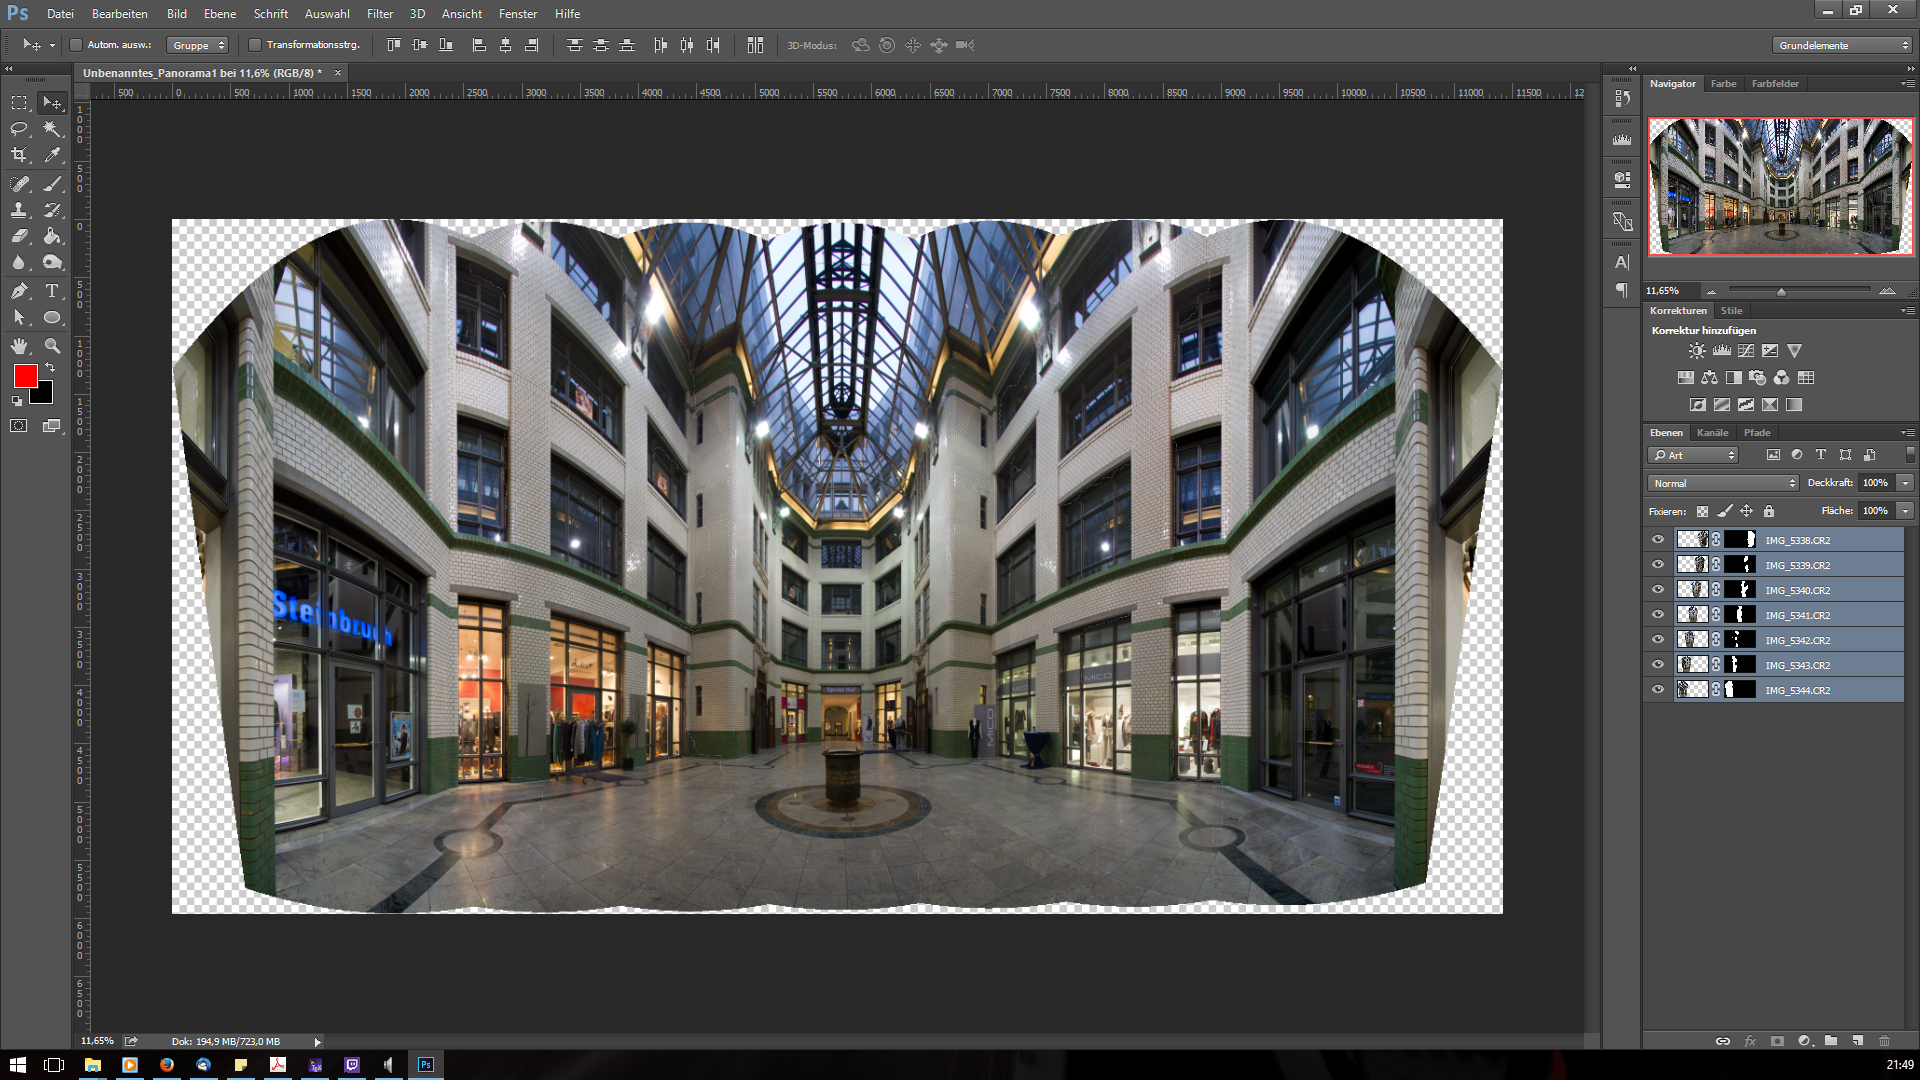
\includegraphics[width=\linewidth]{img/steps/Photoshop_Step_3.png}
		\caption{Photomerge: Speck\grq s Hof}
		\label{img:photoshop_step_3}
	\end{figure}
	\bigskip
	Anders verhält es sich bei komplexeren Panoramen, wie z. B. bei dem Kugelpanorama der Mädler--Passage (s. Abb. \ref{img:photoshop_step_kugel}). Photomerge ist es nicht gelungen die Bilder in der richtigen Reihenfolge zusammenzusetzen. Da das Tool keine Möglichkeit einer Korrektur, Nachjustierung oder Neuanordnung bietet, kann das Panorama nicht damit umgesetzt werden.
	\begin{figure}[H]
		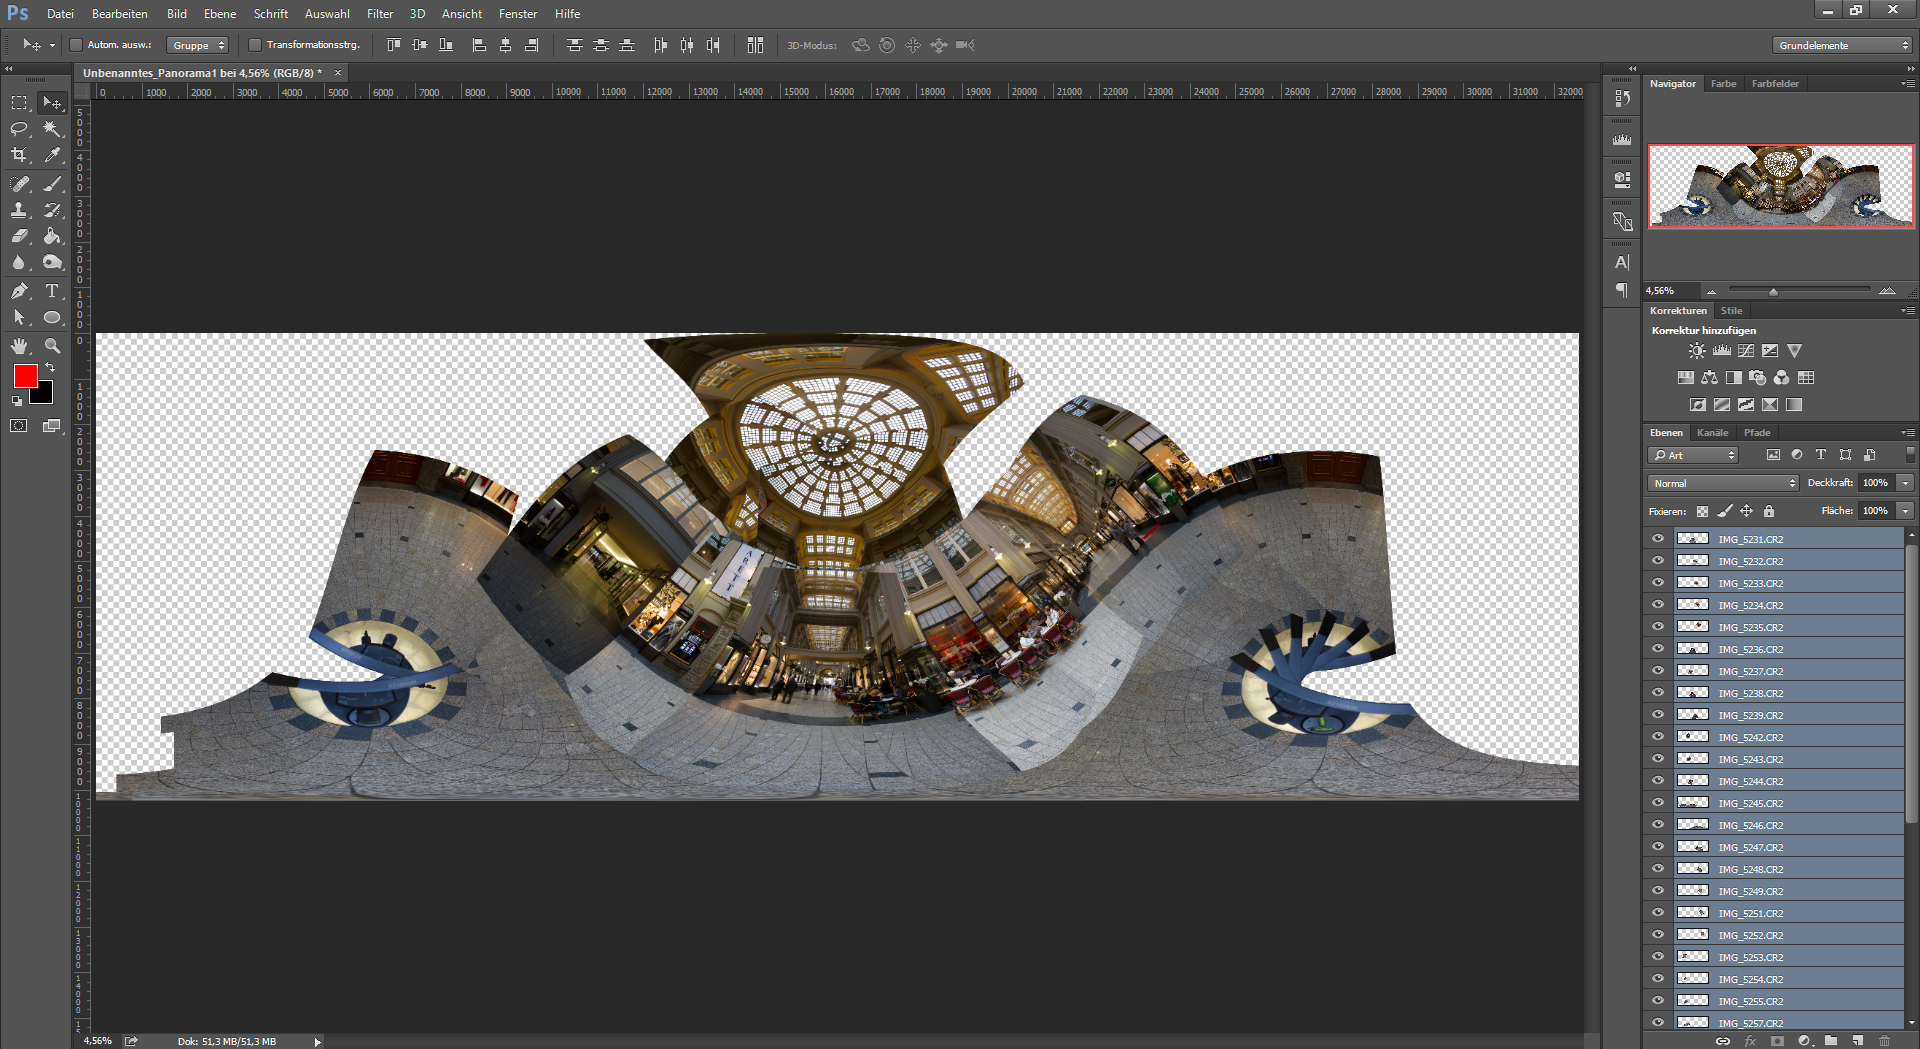
\includegraphics[width=\linewidth]{img/steps/Photoshop_Step_Kugel.png}
		\caption{Photomerge: Kugelpanorama}
		\label{img:photoshop_step_kugel}
	\end{figure}
	\bigskip
	Photoshop eignet sich daher für einfache Panoramen mit einer Ebene. Sobald die Anordnung der Fotos komplexer wird oder manuelle Korrekturen vorgenommen werden müssen, sollte auf eine Spezialsoftware zurückgegriffen werden.  
	
	\chapter{Nachbearbeitung}
	\label{ch:nach}
	Bei der Nachbearbeitung ist es wichtig darauf zu achten, möglichst verlustfreie Formate zu importieren. Auf diese Weise ist garantiert, dass die Bildqualität bei der Bearbeitung nicht so stark abnimmt, wie das bei den komprimierten Formaten, wie jpg der Fall ist. Bei diesem Projekt werden daher ausschließlich Panoramen im TIFF-Format bearbeitet und exportiert.
	
	\section{Adobe Photoshop}
	\label{sec:photo}
	Nach dem Export aus PTGui Pro, wird jedes Panorama mit Photoshop geöffnet. In dieser Software können störende Elemente, wie z. B. fehlende Pflastersteine oder Wolkenformationen, Blätter, Müll oder Personen entfernt werden. Dazu bietet Photoshop Tools, wie den Bereichsreparaturpinsel oder das Stempelwerkzeug. Diese sind in der Lage automatisiert inhaltsbasierte Korrekturen vorzunehmen. Auch wird bei diesem Vorgang bereits der Bildausschnitt gewählt und transparente Flächen abgeschnitten oder aufgefüllt.
	\bigskip
	Bei dem Kugelpanorama der Mädler--Passage (s. Abb. \ref{img:photoshop_step_kugel}) wird das Stativ durch das Überlagern eines stativfreien Fotos mittels Photoshop entfernt s. Abb. \ref{img:photoshop_bearbeitung}. Zudem wird die Spiegelung des Fotografen nachträglich entfernt.  
	
	\begin{figure}[H]
		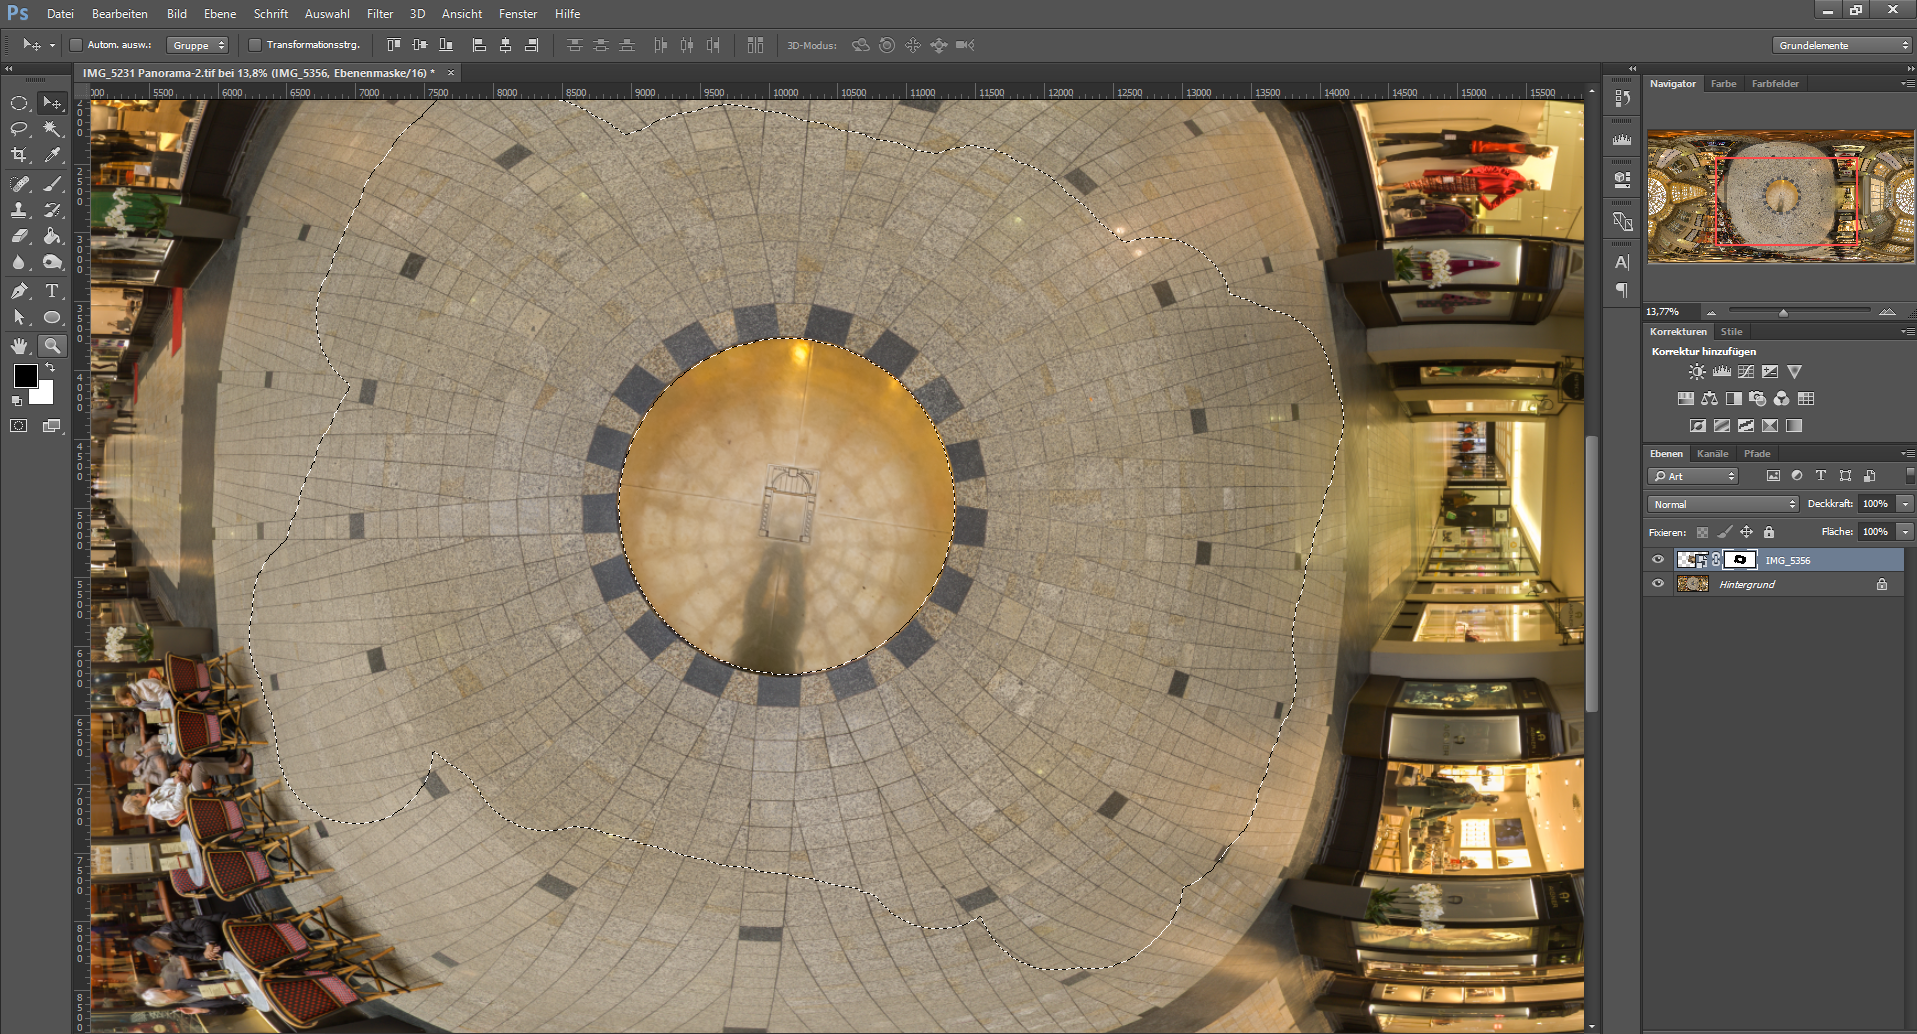
\includegraphics[width=\linewidth]{img/steps/PS_Kugel_Edit.PNG}
		\caption{Photoshop: Nachbearbeitung}
		\label{img:photoshop_bearbeitung}
	\end{figure}
	
	\section{Adobe Lightroom}
	\label{sec:lightroom}
	Lightroom stammt auch aus dem Hause Adobe und dient hauptsächlich Verwaltung und Nachbearbeitung von Fotos. So erkennt die Software automatisch die meisten Kameramodelle und bietet entsprechende Entzerrungs- und Korrekturoptionen an. So ist beispielsweise möglich, Abberationen automatisiert zu entfernen. In diesem Projekt wird vorerst der Weißabgleich angepasst und anschließend die Tiefen und Höhen bearbeitet. Die Lichter und der Weißwert müssen so angeglichen werden, dass es möglichst keine ausgebrannten Stellen gibt. Zusätzlich erfolgt die Korrektur von Kontrast, Sättigung und Schärfe. in der Abbildung \ref{img:lightroom_bearbeitung} wird ein solcher Korrekturvorgang beispielhaft veranschaulicht. Zum Schluss erfolgt, falls nötig, nochmals die Auswahl des richtigen Bildausschnittes.
	\begin{figure}[H]
		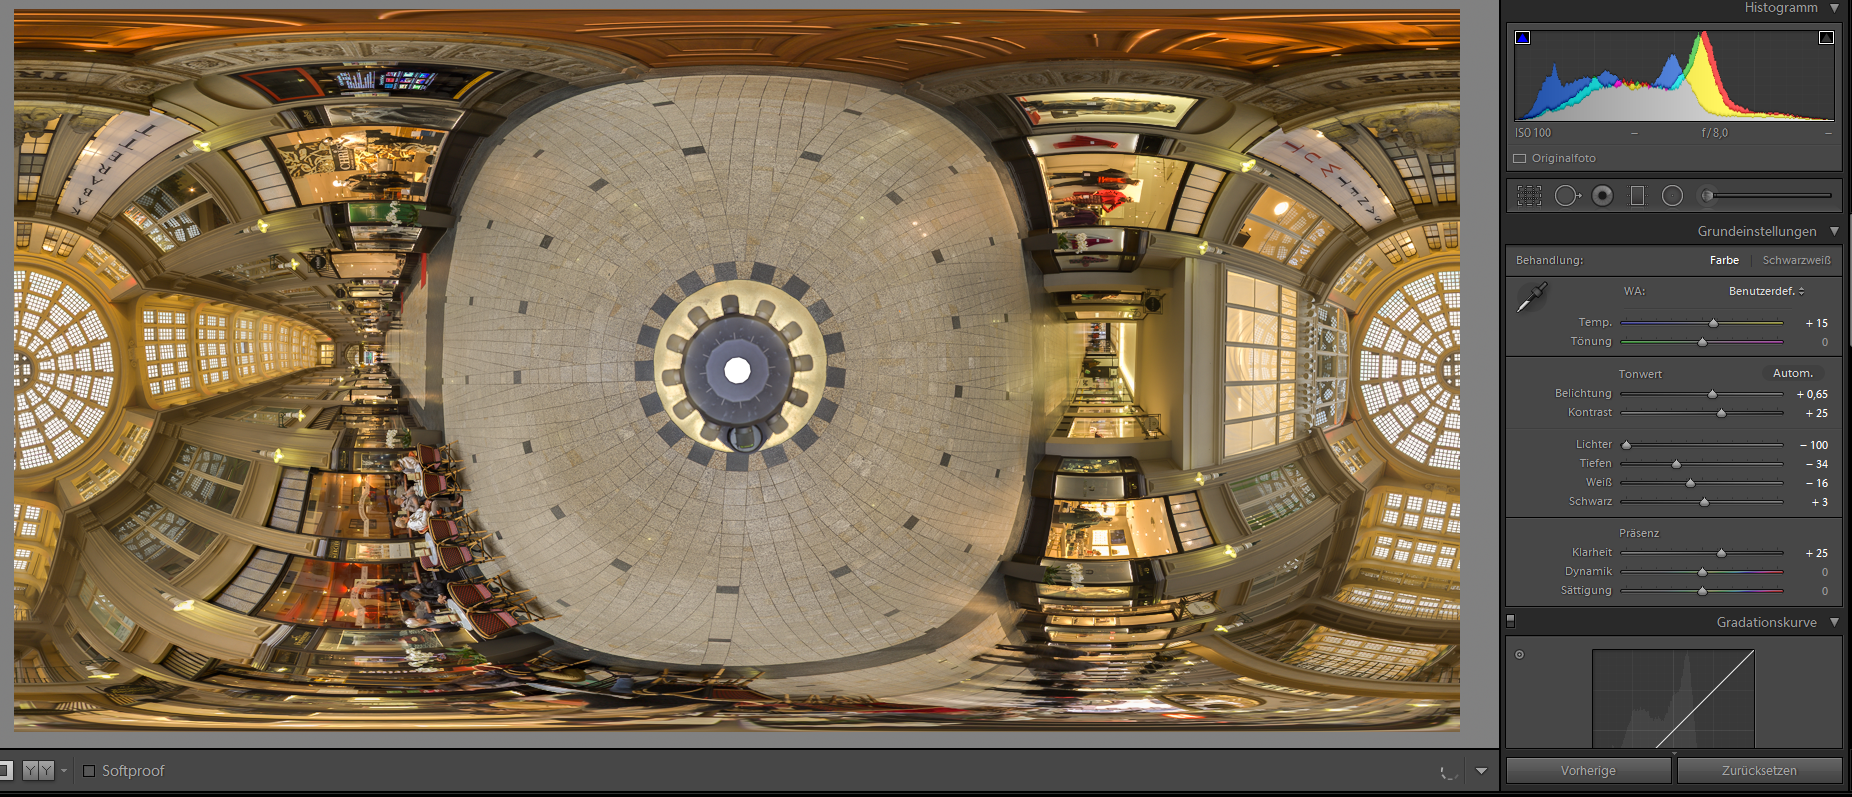
\includegraphics[width=\linewidth]{img/steps/Lightroom_kugel.PNG}
		\caption{Lightroom: Nachbearbeitung}
		\label{img:lightroom_bearbeitung}
	\end{figure}

	
	\begin{thebibliography}{999}
	
		
	\end{thebibliography}
	
\end{document}